\newpage
\section{Results}
\label{sec:results}

Here below a brief enumeration of the achieved results during this project.
\\
\\
a) A designed and implemented mathematical model to detect geospatial-temporal commuting patterns.
\\
\\
b) A set of charts and maps which illustrate the previous model, making easier to deduce interesting findings.
\\
\\
c) An on-line application\footnote{"Poner la dirección de las herramientas"} to display all this information in a friendly and customizable way.
\\
\\
Now, let's describe deeply them, as well as other partial findings.
\\
\\
According to the proposed model, a very important feature has been deduced for the Commuting Dynamic. As seen in the picture below, there are two time zones when people perform more phone calls from their handsets than usual. Static and dynamic users have not been distinguished, that is, both self-edges and transition edges are counted together.

\begin{figure}[h]
\begin{center}
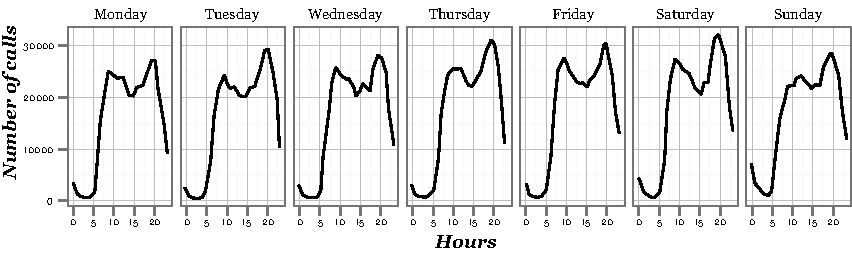
\includegraphics[scale =1.1] {results/images/calls_number.pdf}
\caption{Total amount of calls grouped by Week days}
\label{fig:count_calls}
\end{center}
\end{figure}


There are two peaks, $p_1$, from 7:00 am to 9:00 am, and another one, $p_2$, from 6:00 pm to 8:00 pm. As it can be seen, the 'morning-peak' is lower than the 'evening-peak'. Moreover, both peaks reach their maximum value at the end of their corresponding time zones, i.e., $p_1$ at 9:30 am and $p_2$ at 7:30 pm. Note how the amount of calls increases linearly since 5 am and how it decreases linearly too since 8:00 pm. Another remarkable feature is the existence of a central valley between $p_1$ and $p_2$, that is, from 9:00 am to 6:00 pm. This 'peak-valley-peak' pattern is shown for all days in the week, so that it can be assumed that people have the same behaviour (at least, according to our target datasets).
\\
\\
Let's extract some ideas from the previous chart, focusing on what commuters could be probably doing (as it will be seen shortly, most of the phone calls belong to 'dynamic users'): they get up early in the morning and start to perform more and more phone calls from their handsets until $p1_$; next, the amount of phone calls decreases slightly, keeping itself more or less balanced (workhours, lunch) until the beginning of $p2_$; later, people leave the office and plan the rest of the day (errands, leisure...), what is reflected on a marked rise in the amount of phone calls.
\\
\\
Since it is really complicated to measure the displacements of the people (antenna locations instead of users locations, missing antena identifiers...), what will be analyzed is the amount of callers who are really commuters, that is, dynamic users. This one will be the essential magnitude of our research, leading us to figure out the Commuting Dynamics key-features for different regions and times. Eventually, all conclusions deduced from the G/T Model (charts, formulae...) will be ultimately tested with the final GIS visualization as the main core of the work. In this last phase, geographical displacements are estimated so that they can be plotted in a dynamic and interactive map which makes easier to detect peaks and trends.
\\
\\
With this new chart, it is the ratio between commuters and all users what it is being emphasized. During a particular day (24h), there is no need to know if a concrete displacement is or not longer than other. What it is being highlighted here is the movement detection itself, in 1h windows which group all users calling within them. The colour of the chart shows how many users are really commuters.
\\
\\
Datasets have been processed according to the proposed G/T Model, filtering non-commuters when commuters tracks have been calculated. Here below, seven charts display Commuting Dynamics for each week-day.
As shown in the results, there is no correlation between the number of dynamic users and the maximum displacement peaks, actually, at the same time the number of dynamic users are growing, the central valley and the two maximum commuting peaks are always presented in the sample.
\\
\\
These seven charts below show a fitter correlation with the theoretical commuting model proposed in this paper (Figure ~\ref{fig:commuting}), displaying two high peaks and a lower central valley. However, more qualitative data is necessary to figure out the performance of the first high peak, because it is not related to the number of dynamic users. Furthermore, a first approach can be applied to say that few dynamic users (in comparision with the mean) travel longer distances in this first peak, specially in  the first uphill to the first peak. This is a common pattern figured out from the proposed model. However, it can be explained because there are people starting their travel from further distances early in the morning, since the most of the people live near their work places and travel nearer distances than the first group.  

\newpage

\begin{figure}[h]
\begin{center}
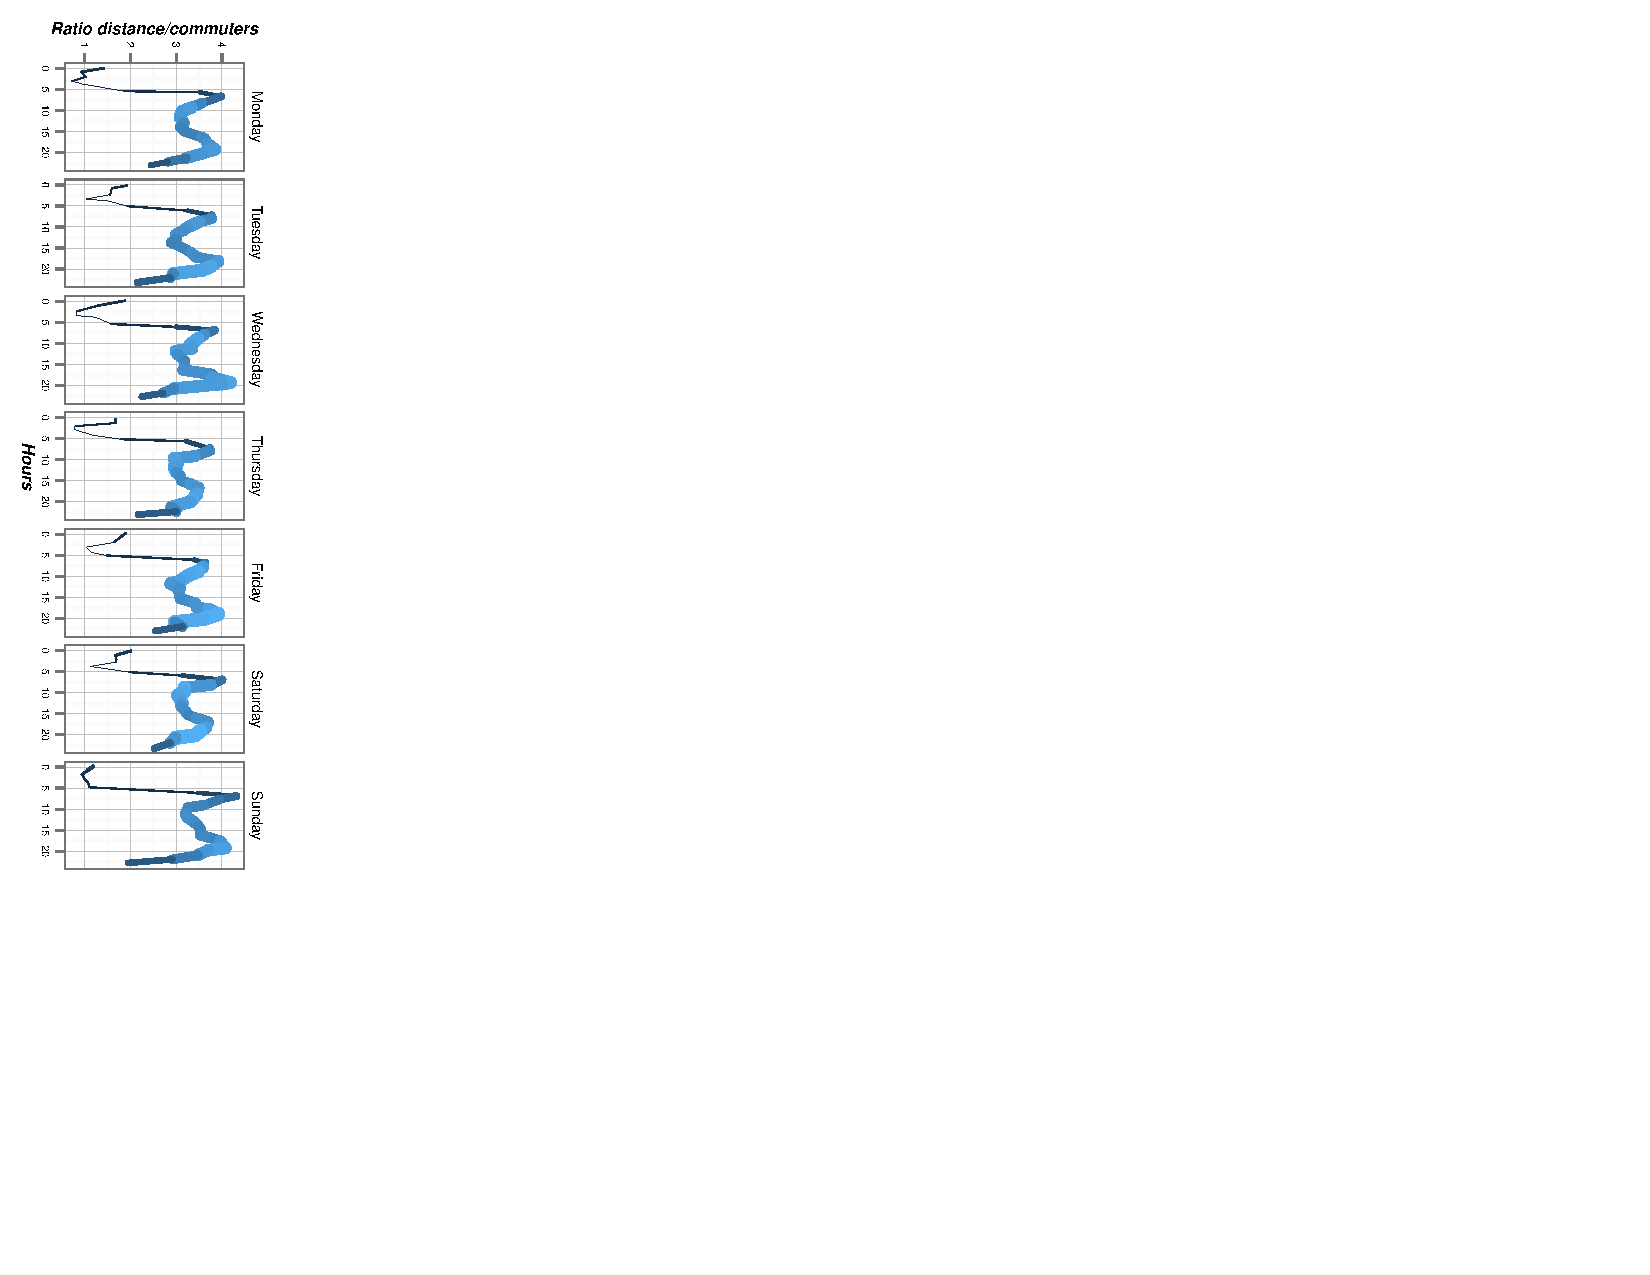
\includegraphics[scale = 0.8] {results/images/commuting_results.pdf}
\caption{Dynamic users displacements}
\label{fig:dynamic_displacements}
\end{center}
\end{figure}

A visualization of the displacement with a Kernel Density estimation using GIS with the antennas positions and users displacements like a directed graph has shown the contraction and the expansion of the commuting dynamics across the 24 hours of the day. The firsts expansion visualization through the kernel density estimation is clearly showed when peak $p_1$ starts to grown between $[5,7]$ reaching the central valley at $8$.

\newpage

\begin{figure}
\centering
\subfigure[Monday, 05:00]{
    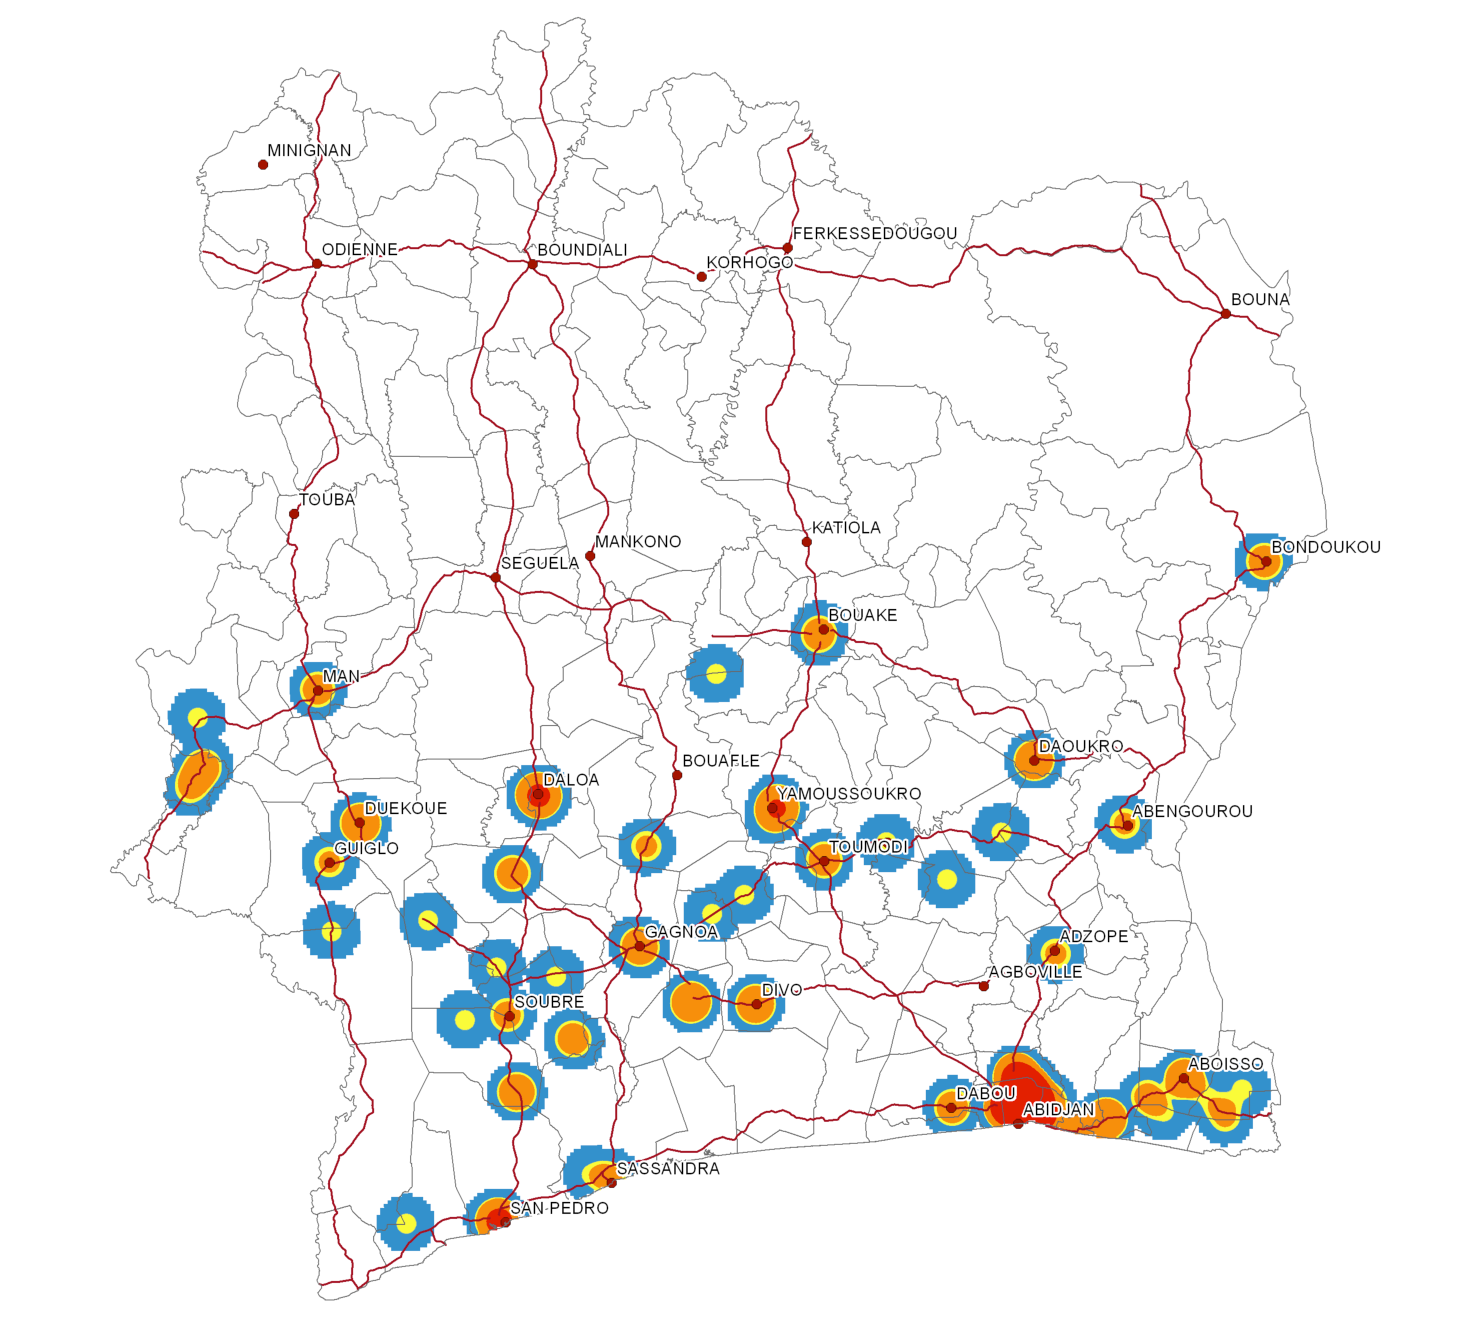
\includegraphics[scale = 0.3]{results/images/kernel/l_hour5_kd.pdf}
	\label{fig:subfig1}
}
\subfigure[Monday, 06:00]{
    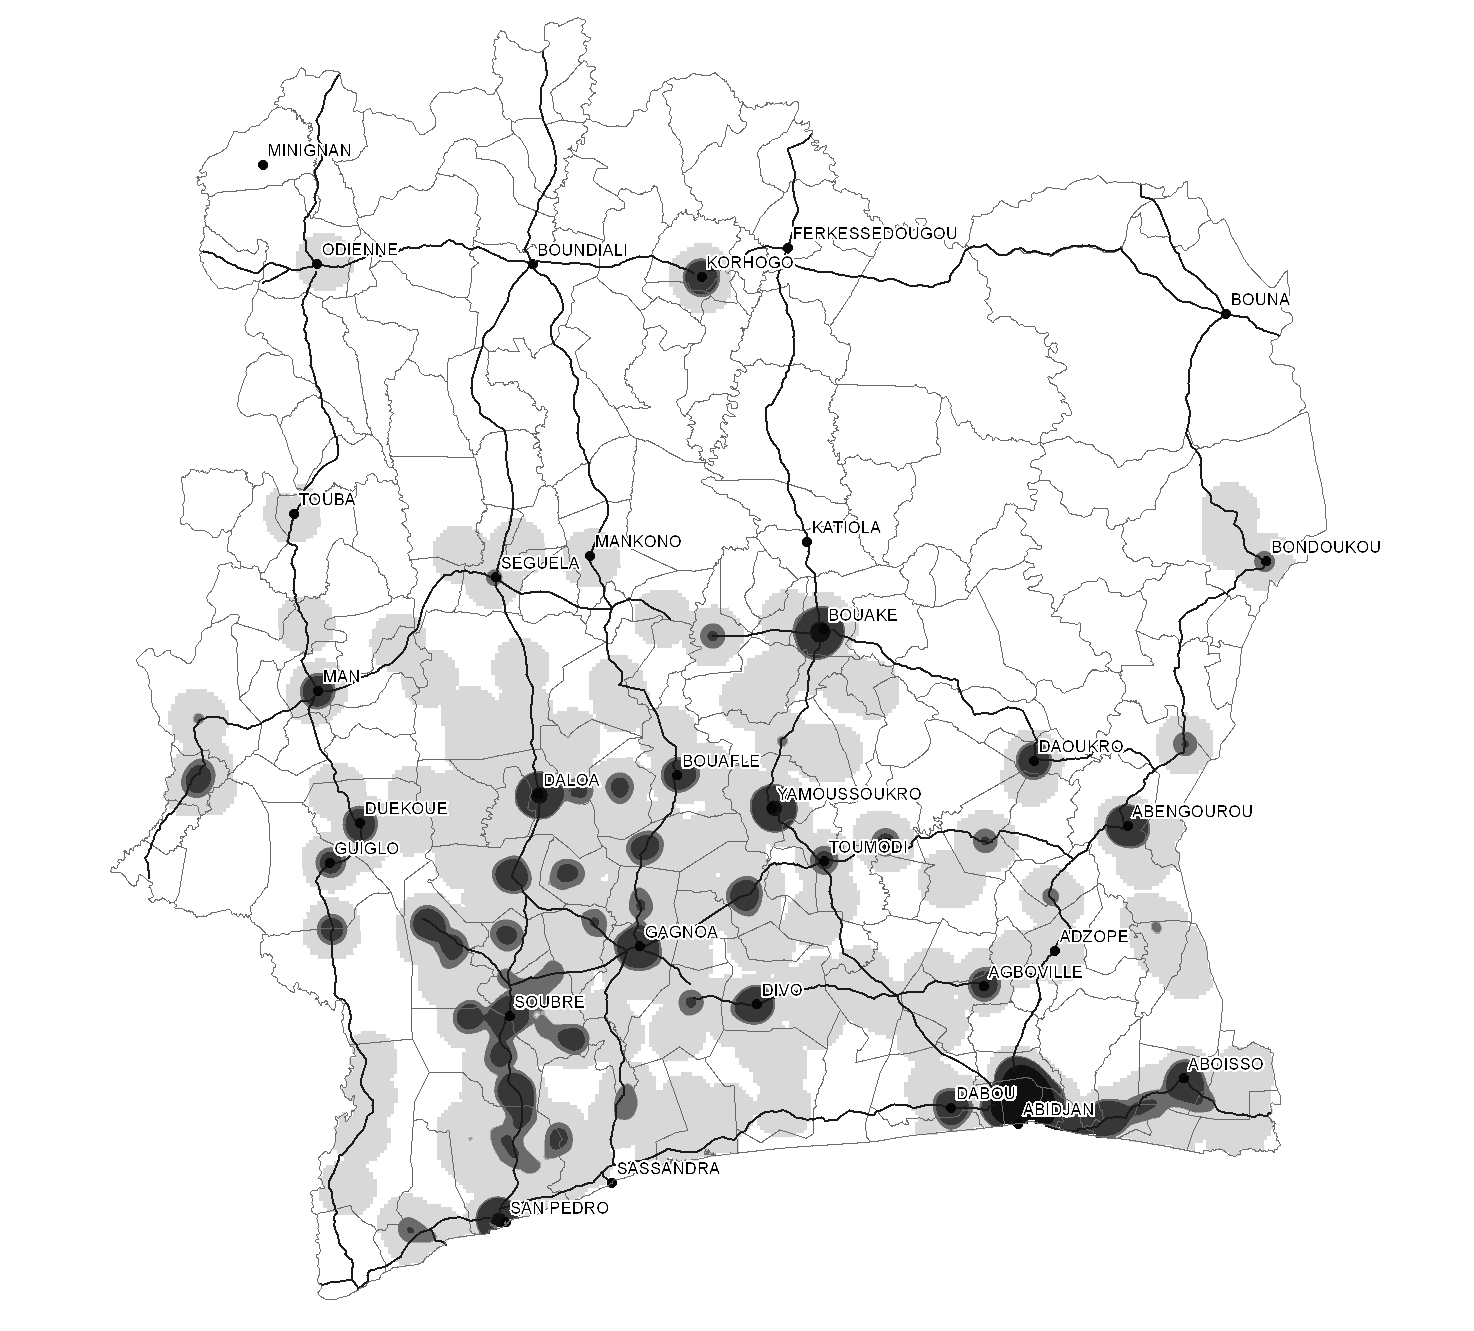
\includegraphics[scale = 0.3]{results/images/kernel/l_hour6_kd.pdf}
	\label{fig:subfig2}
}
\\
\subfigure[Monday, 07:00]{
    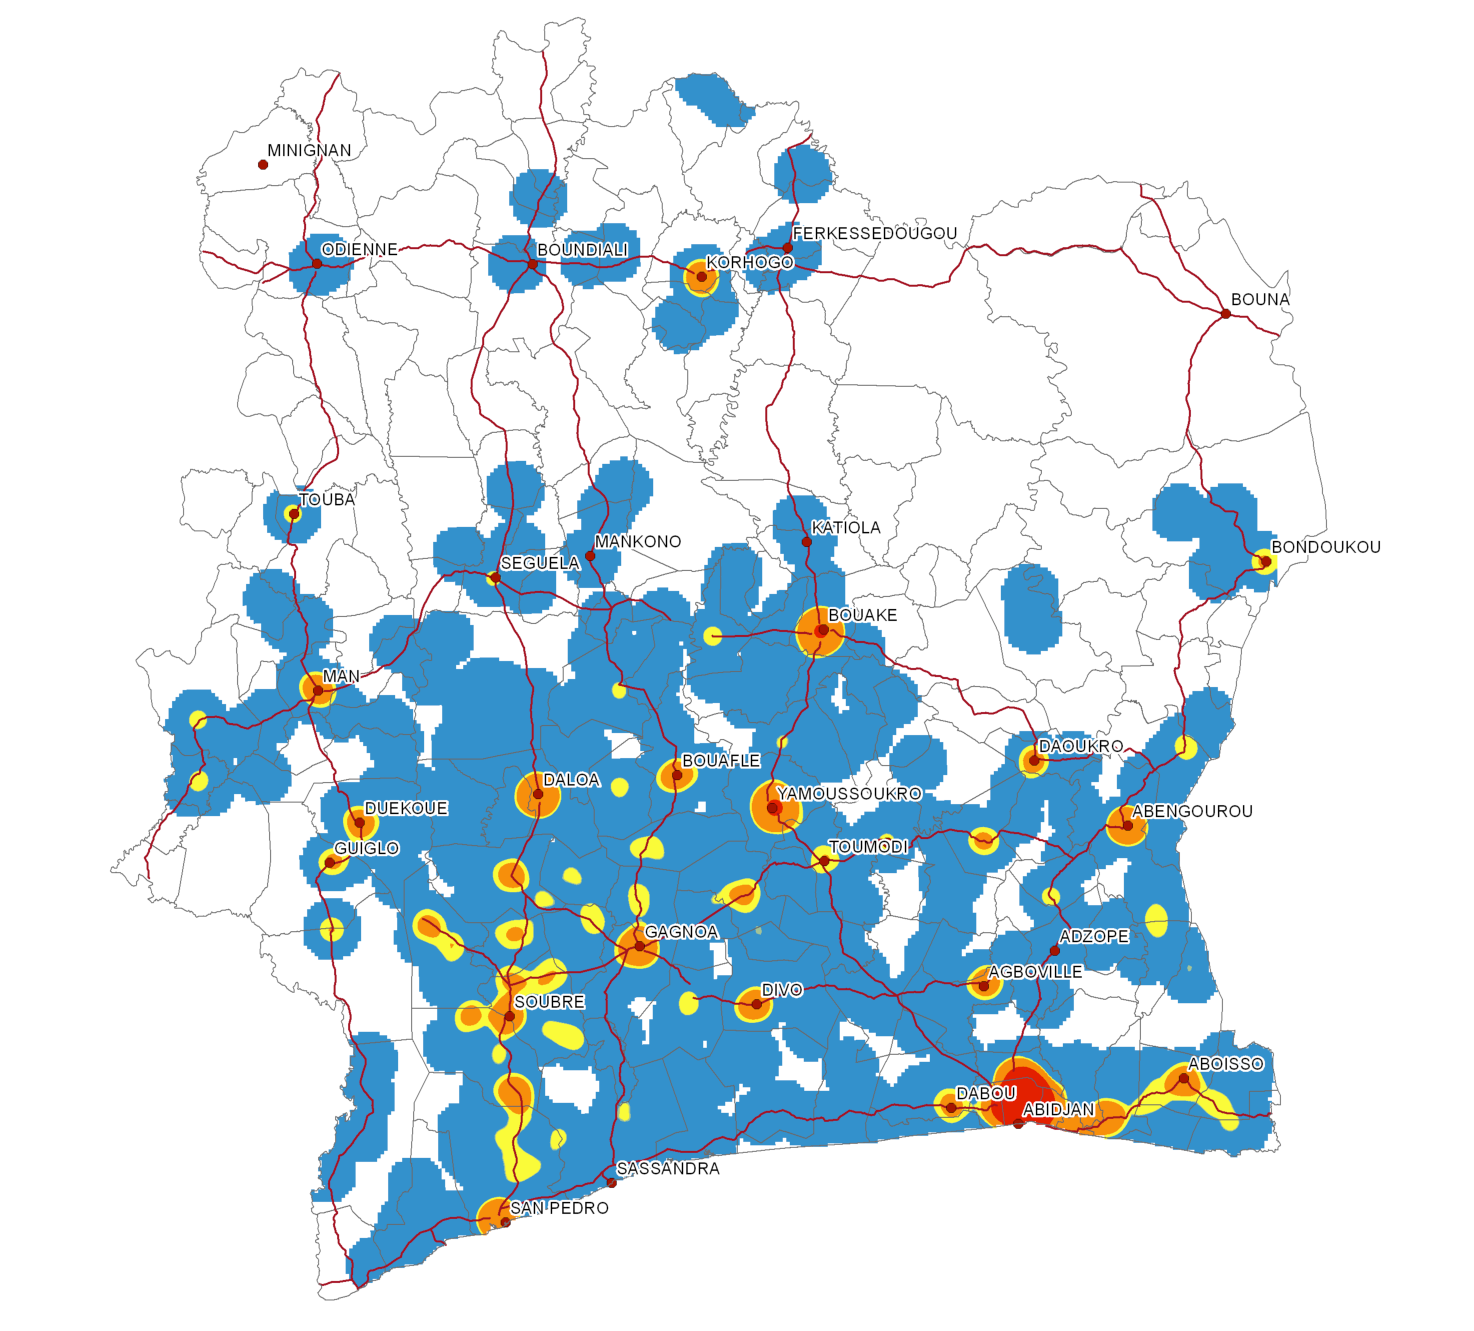
\includegraphics[scale = 0.3]{results/images/kernel/l_hour7_kd.pdf}
	\label{fig:subfig1}
}
\subfigure[Monday, 08:00]{
    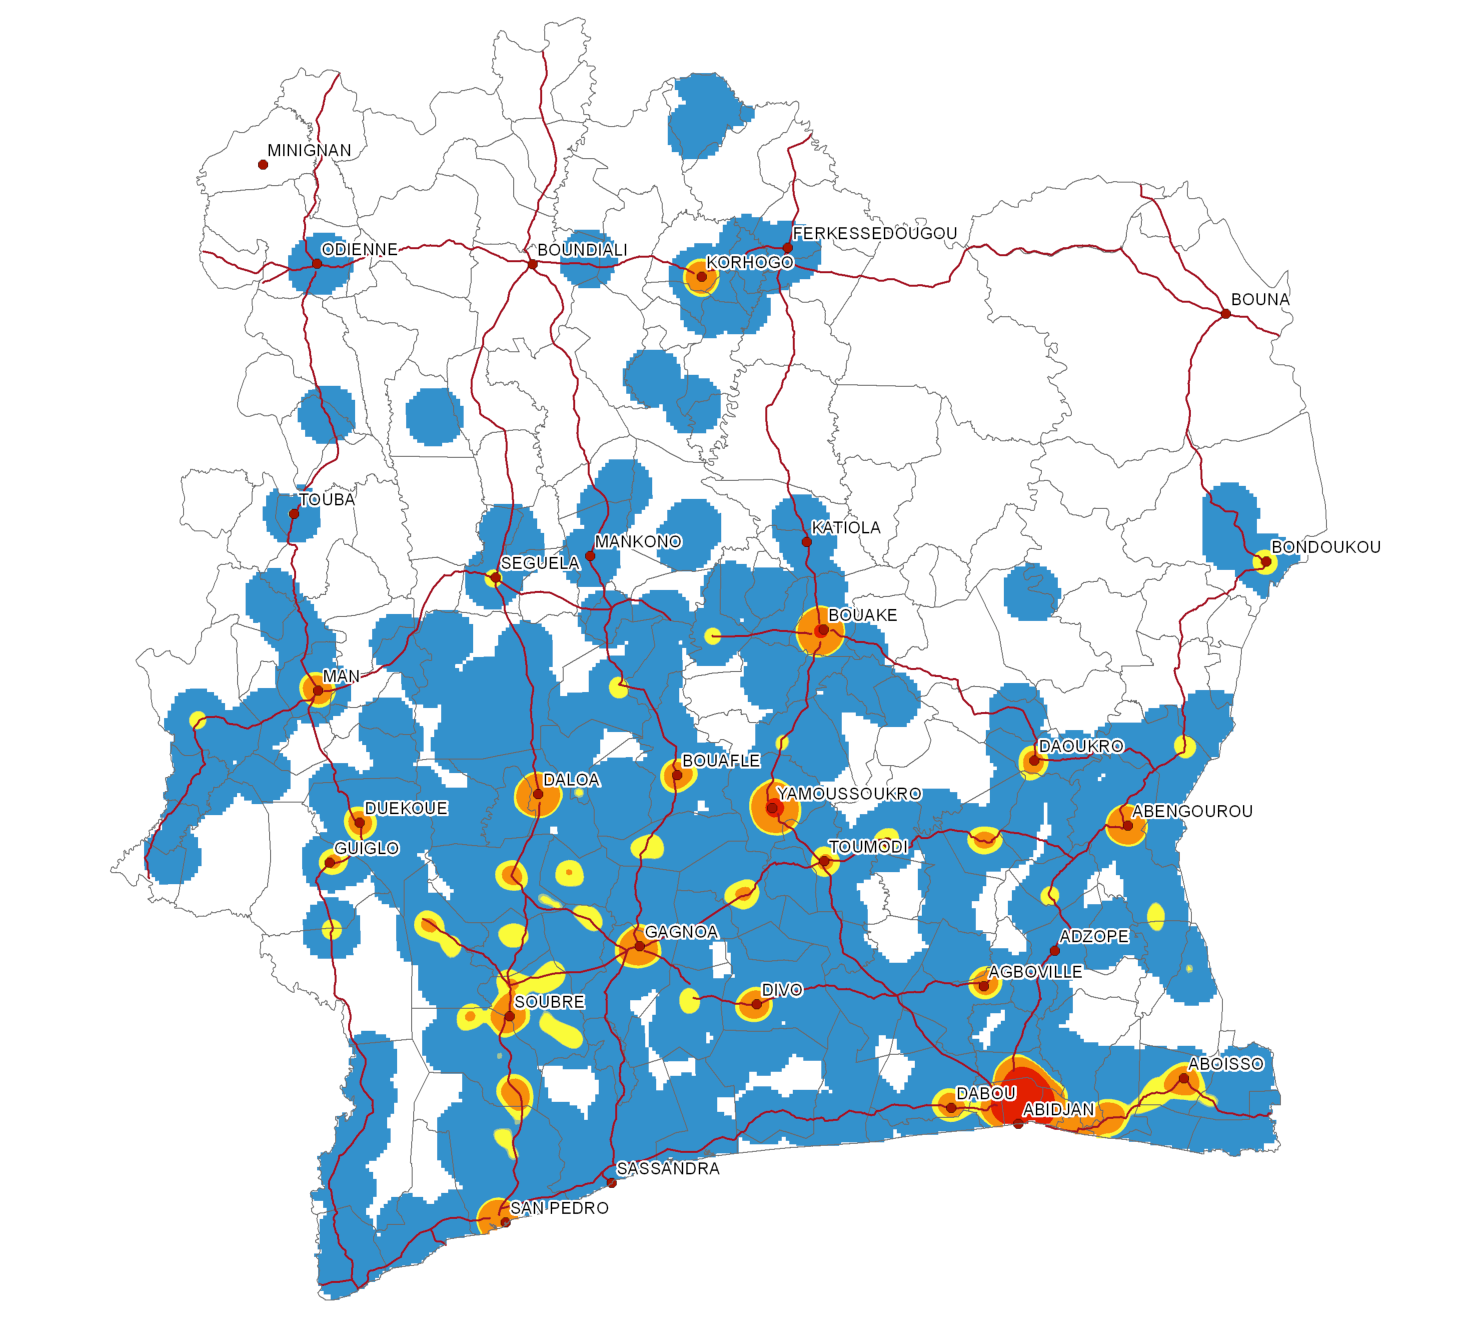
\includegraphics[scale = 0.3]{results/images/kernel/l_hour8_kd.pdf}
	\label{fig:subfig2}
}
\caption[KDE evolution while peak $p_1$ is reached]{Evolution of KDE while peak $p_1$ is reached}
\label{fig:kde_first_peak}
\end{figure}

Also, while a normalize displacement meassure is distributed across the country in the valley hours, a reduction of the displacement of the dynamics users can be appreciated especially on roads where KDE had a high intensity. Above picture,  Monday 06:00, shows cleary a high intensity kernel distributions, coinciding with the maximum displacement moment calculated and showed in the Figure~\ref{fig:dynamic_displacements} on Monday. This values should be identify independently each week day commuting displacement distribution, however, the ranges of peaks $p_1, p_2$ and the central valley are leading for a regular temporal pattern. 
\\
\\
Next pictures shows in a more detailed way the reduction on the KDE on the roads between main cities. We have selected a sample zone in order to show the correlation between the numeric distance calculated by means of the proposed mathematical model in Section~\ref{sec:math_model} and the KDE calculated by means of GIS technology, to test the final aim proposed in this study.
\newpage

\begin{figure}[h!]
\centering
\subfigure[Monday, 05:00]{
    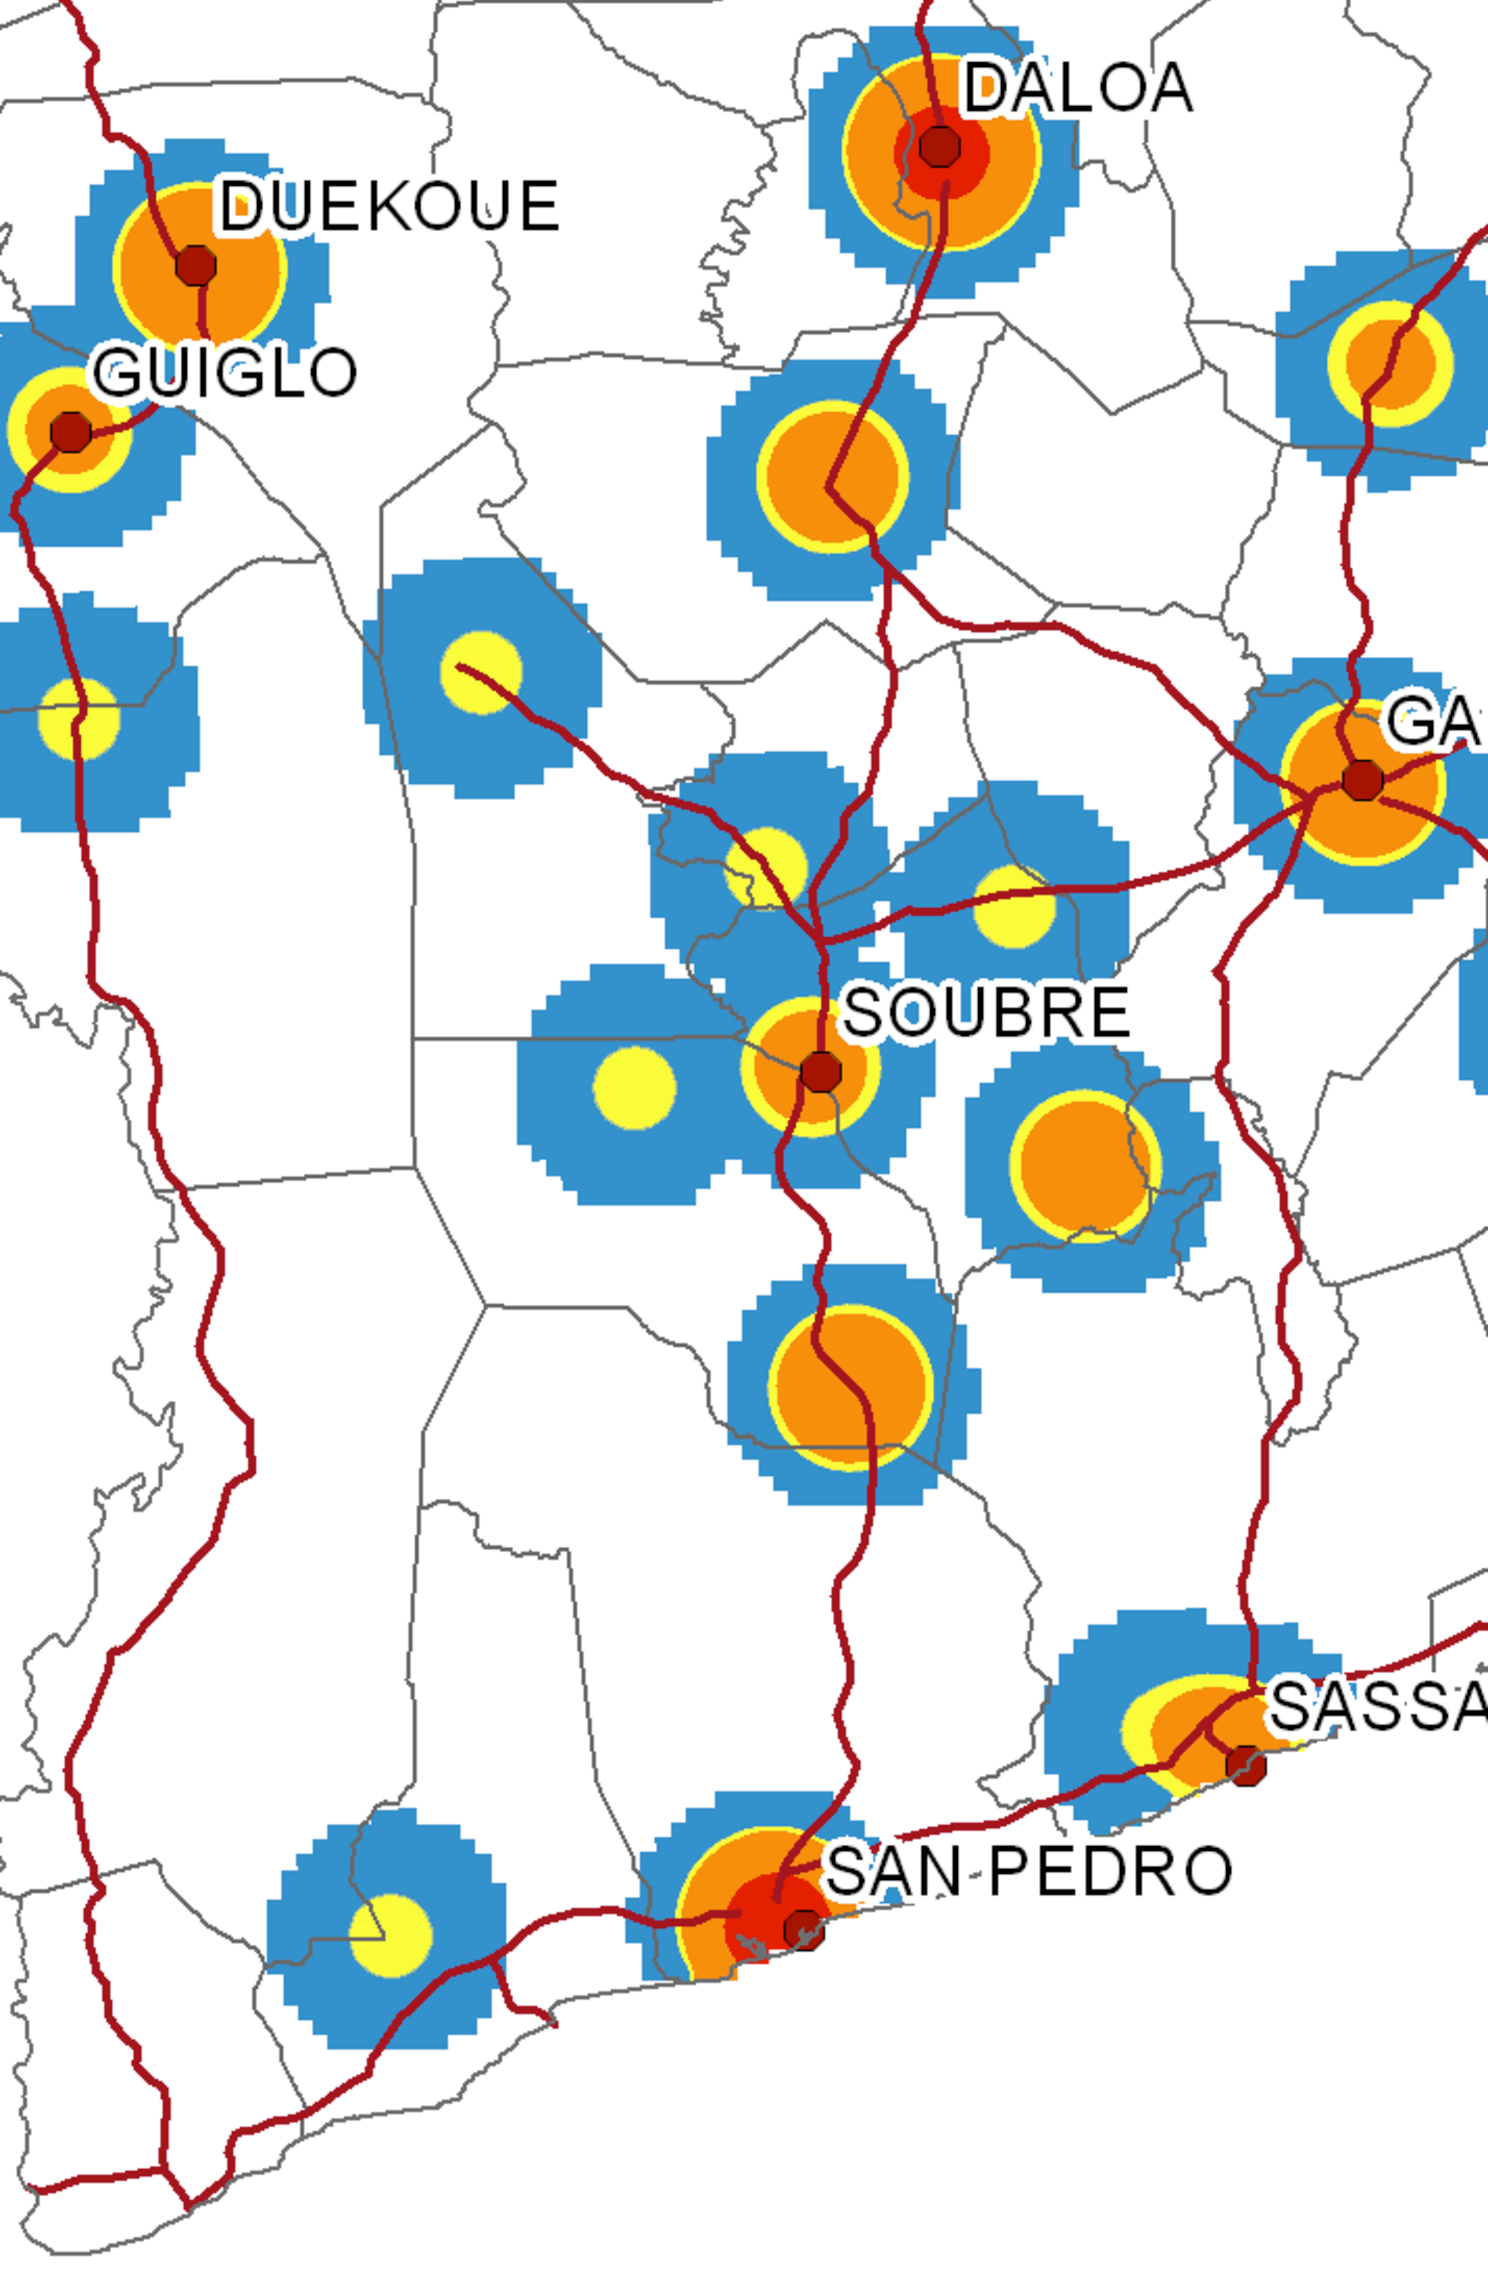
\includegraphics[scale = 0.1]{results/images/kernel/l_hour5_kd_detail.pdf}
	\label{fig:subfig1_detail}
}
\subfigure[Monday, 06:00]{
    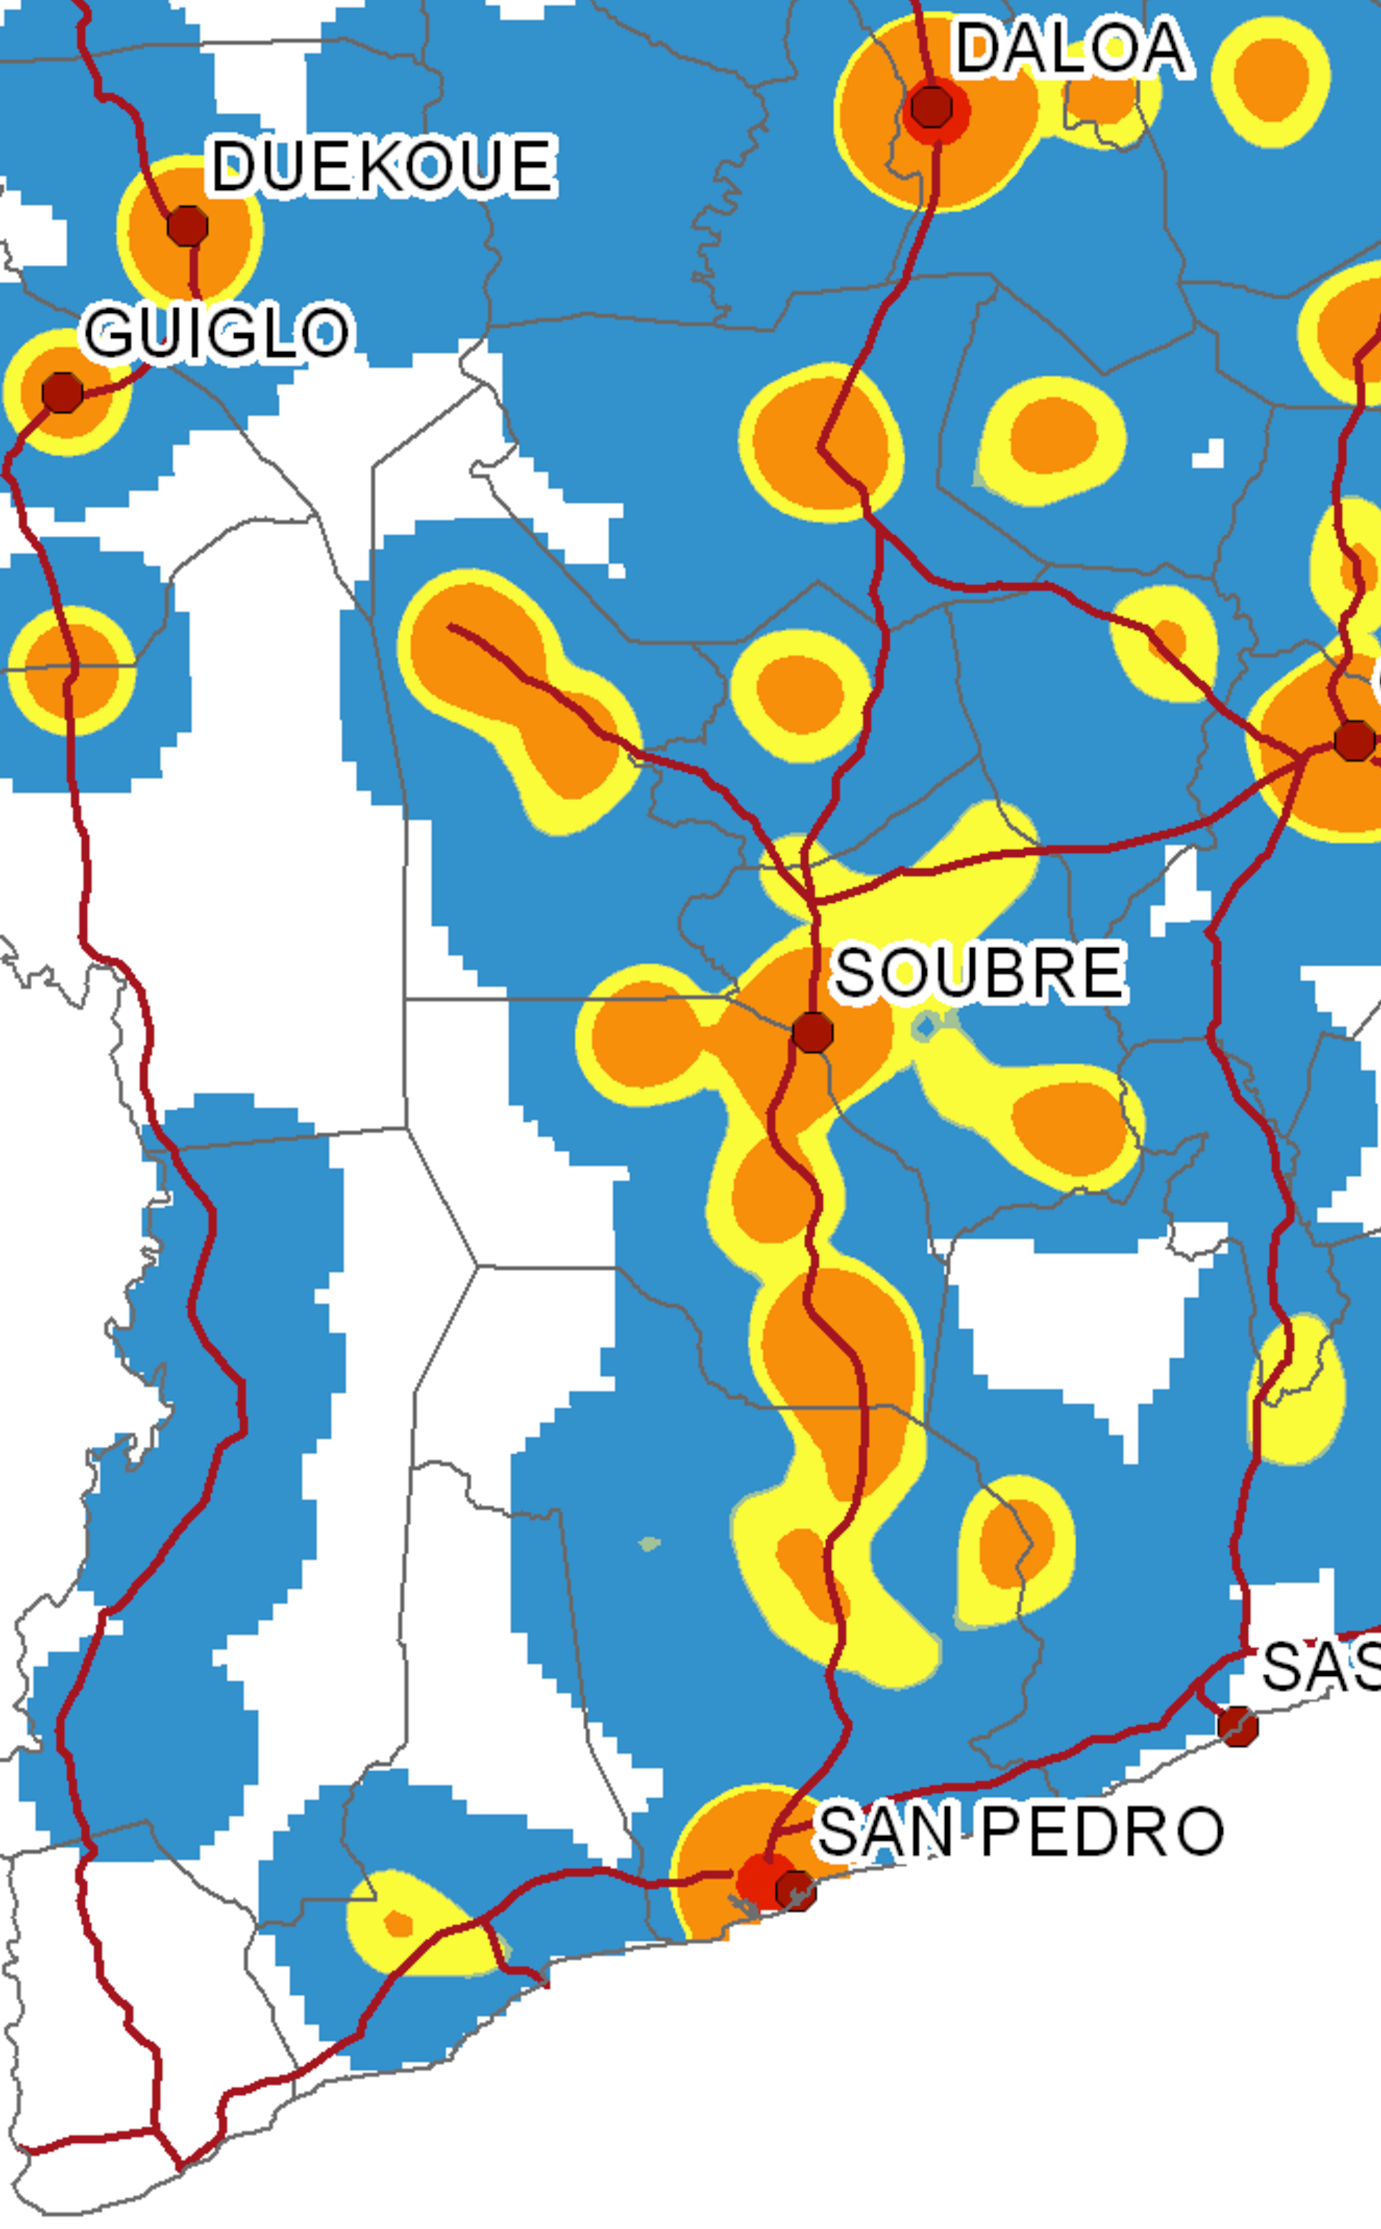
\includegraphics[scale = 0.1]{results/images/kernel/l_hour6_kd_detail.pdf}
	\label{fig:subfig2_detail}
}
\subfigure[Monday, 07:00]{
    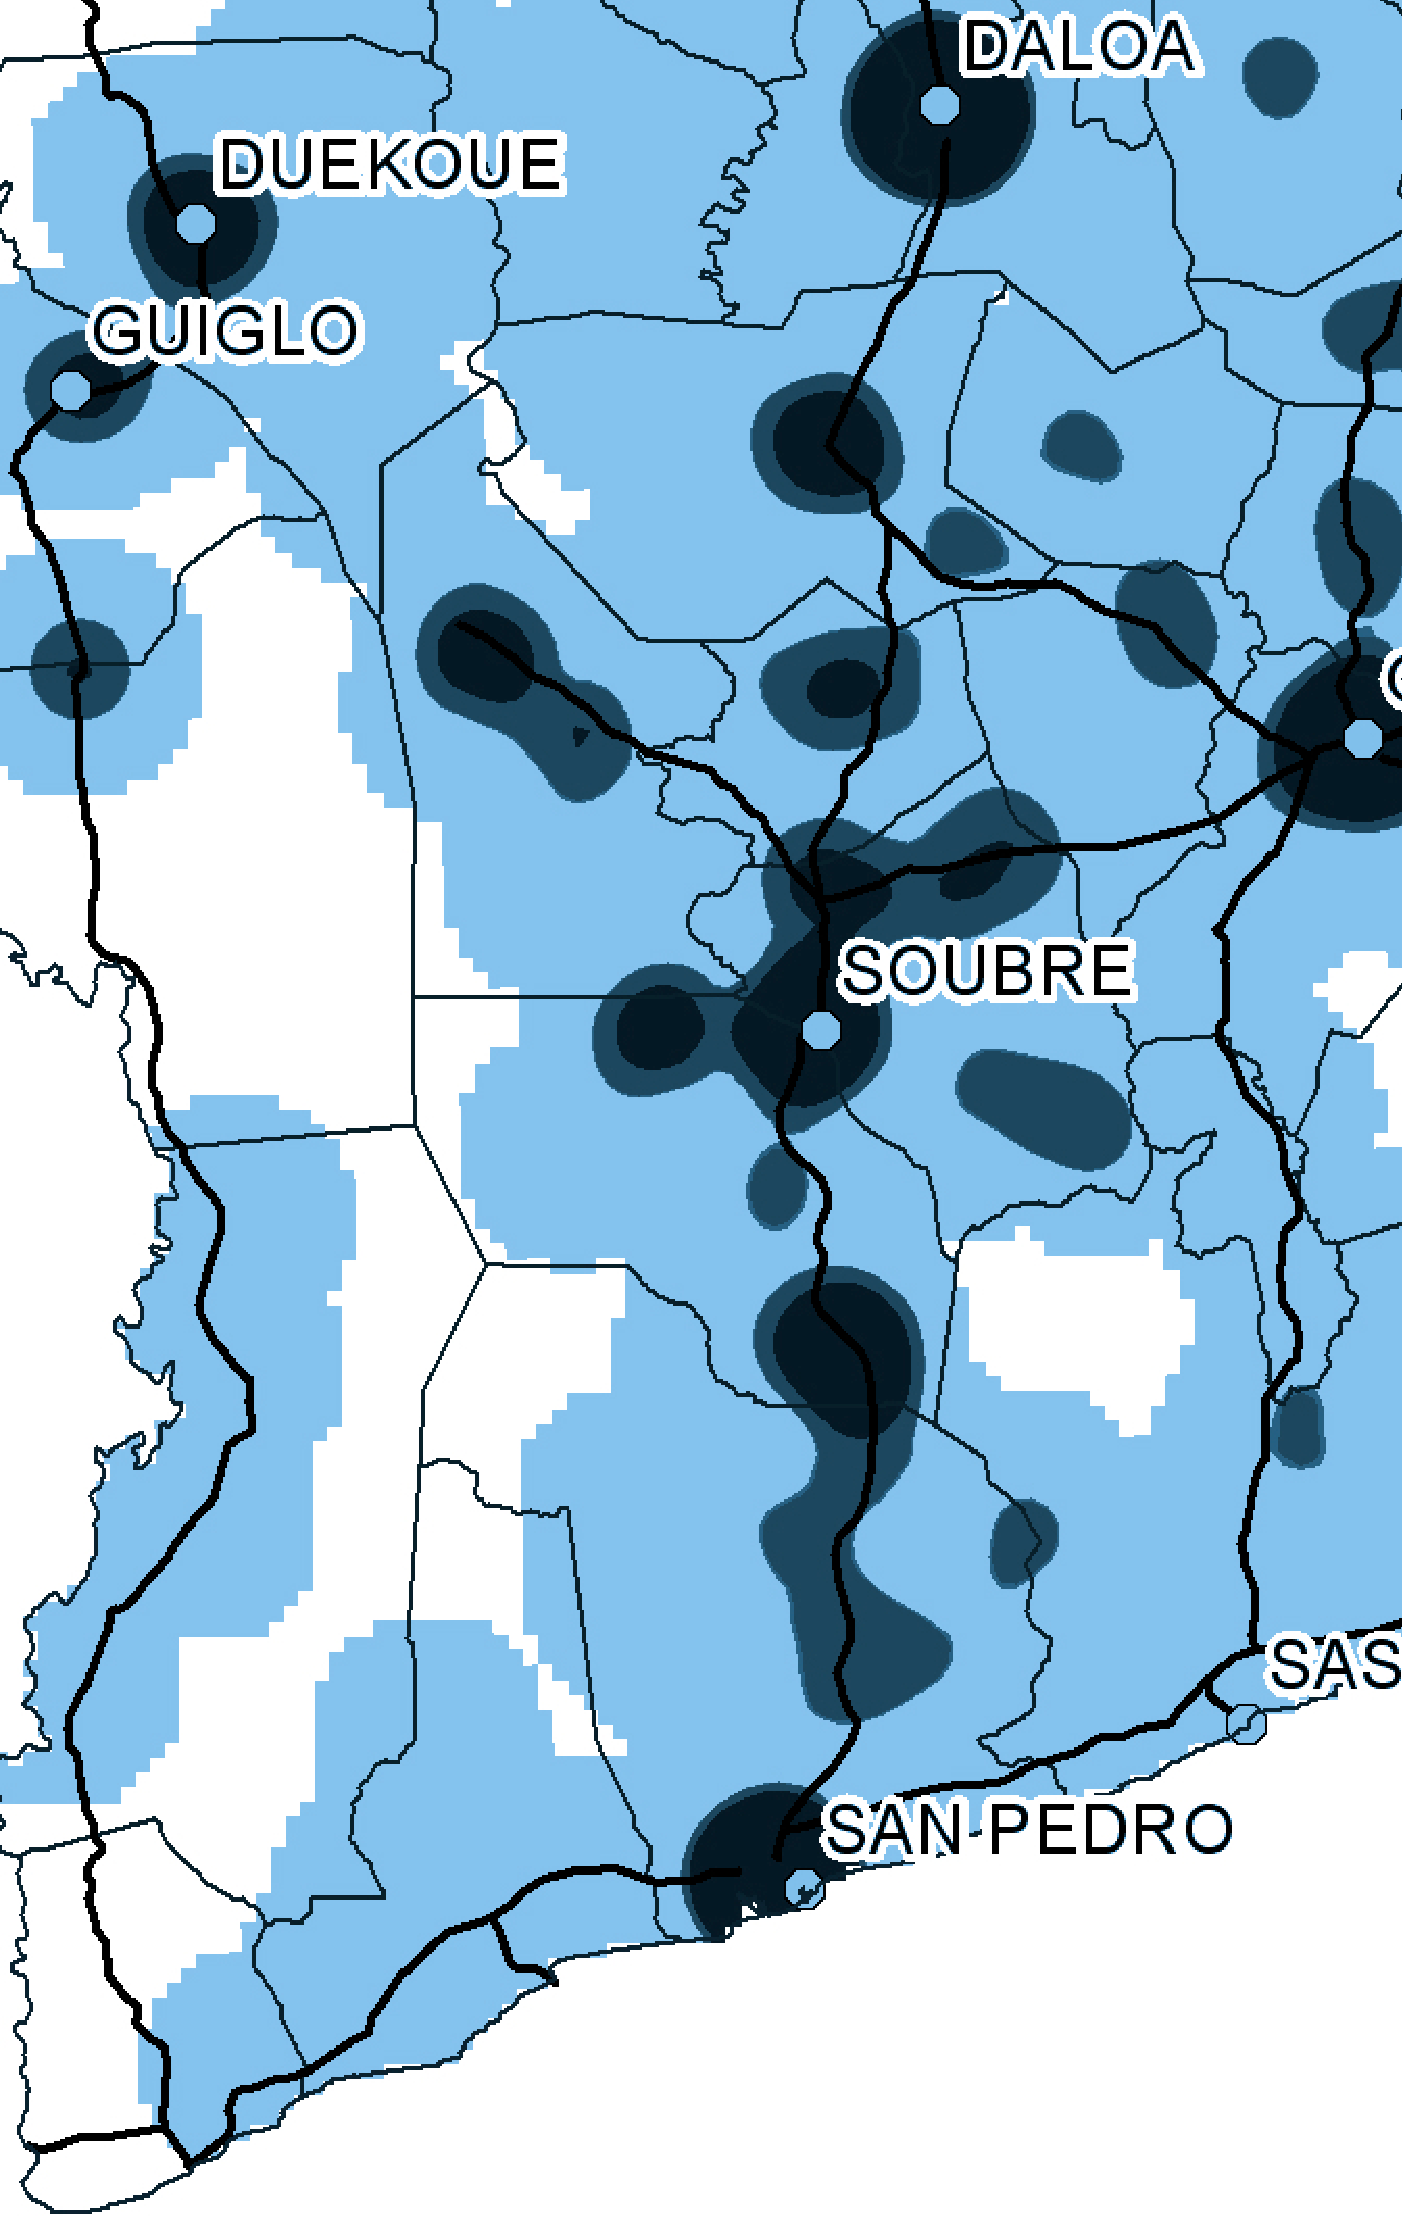
\includegraphics[scale = 0.1]{results/images/kernel/l_hour7_kd_detail.pdf}
	\label{fig:subfig2_detail}
}
\subfigure[Monday, 08:00]{
    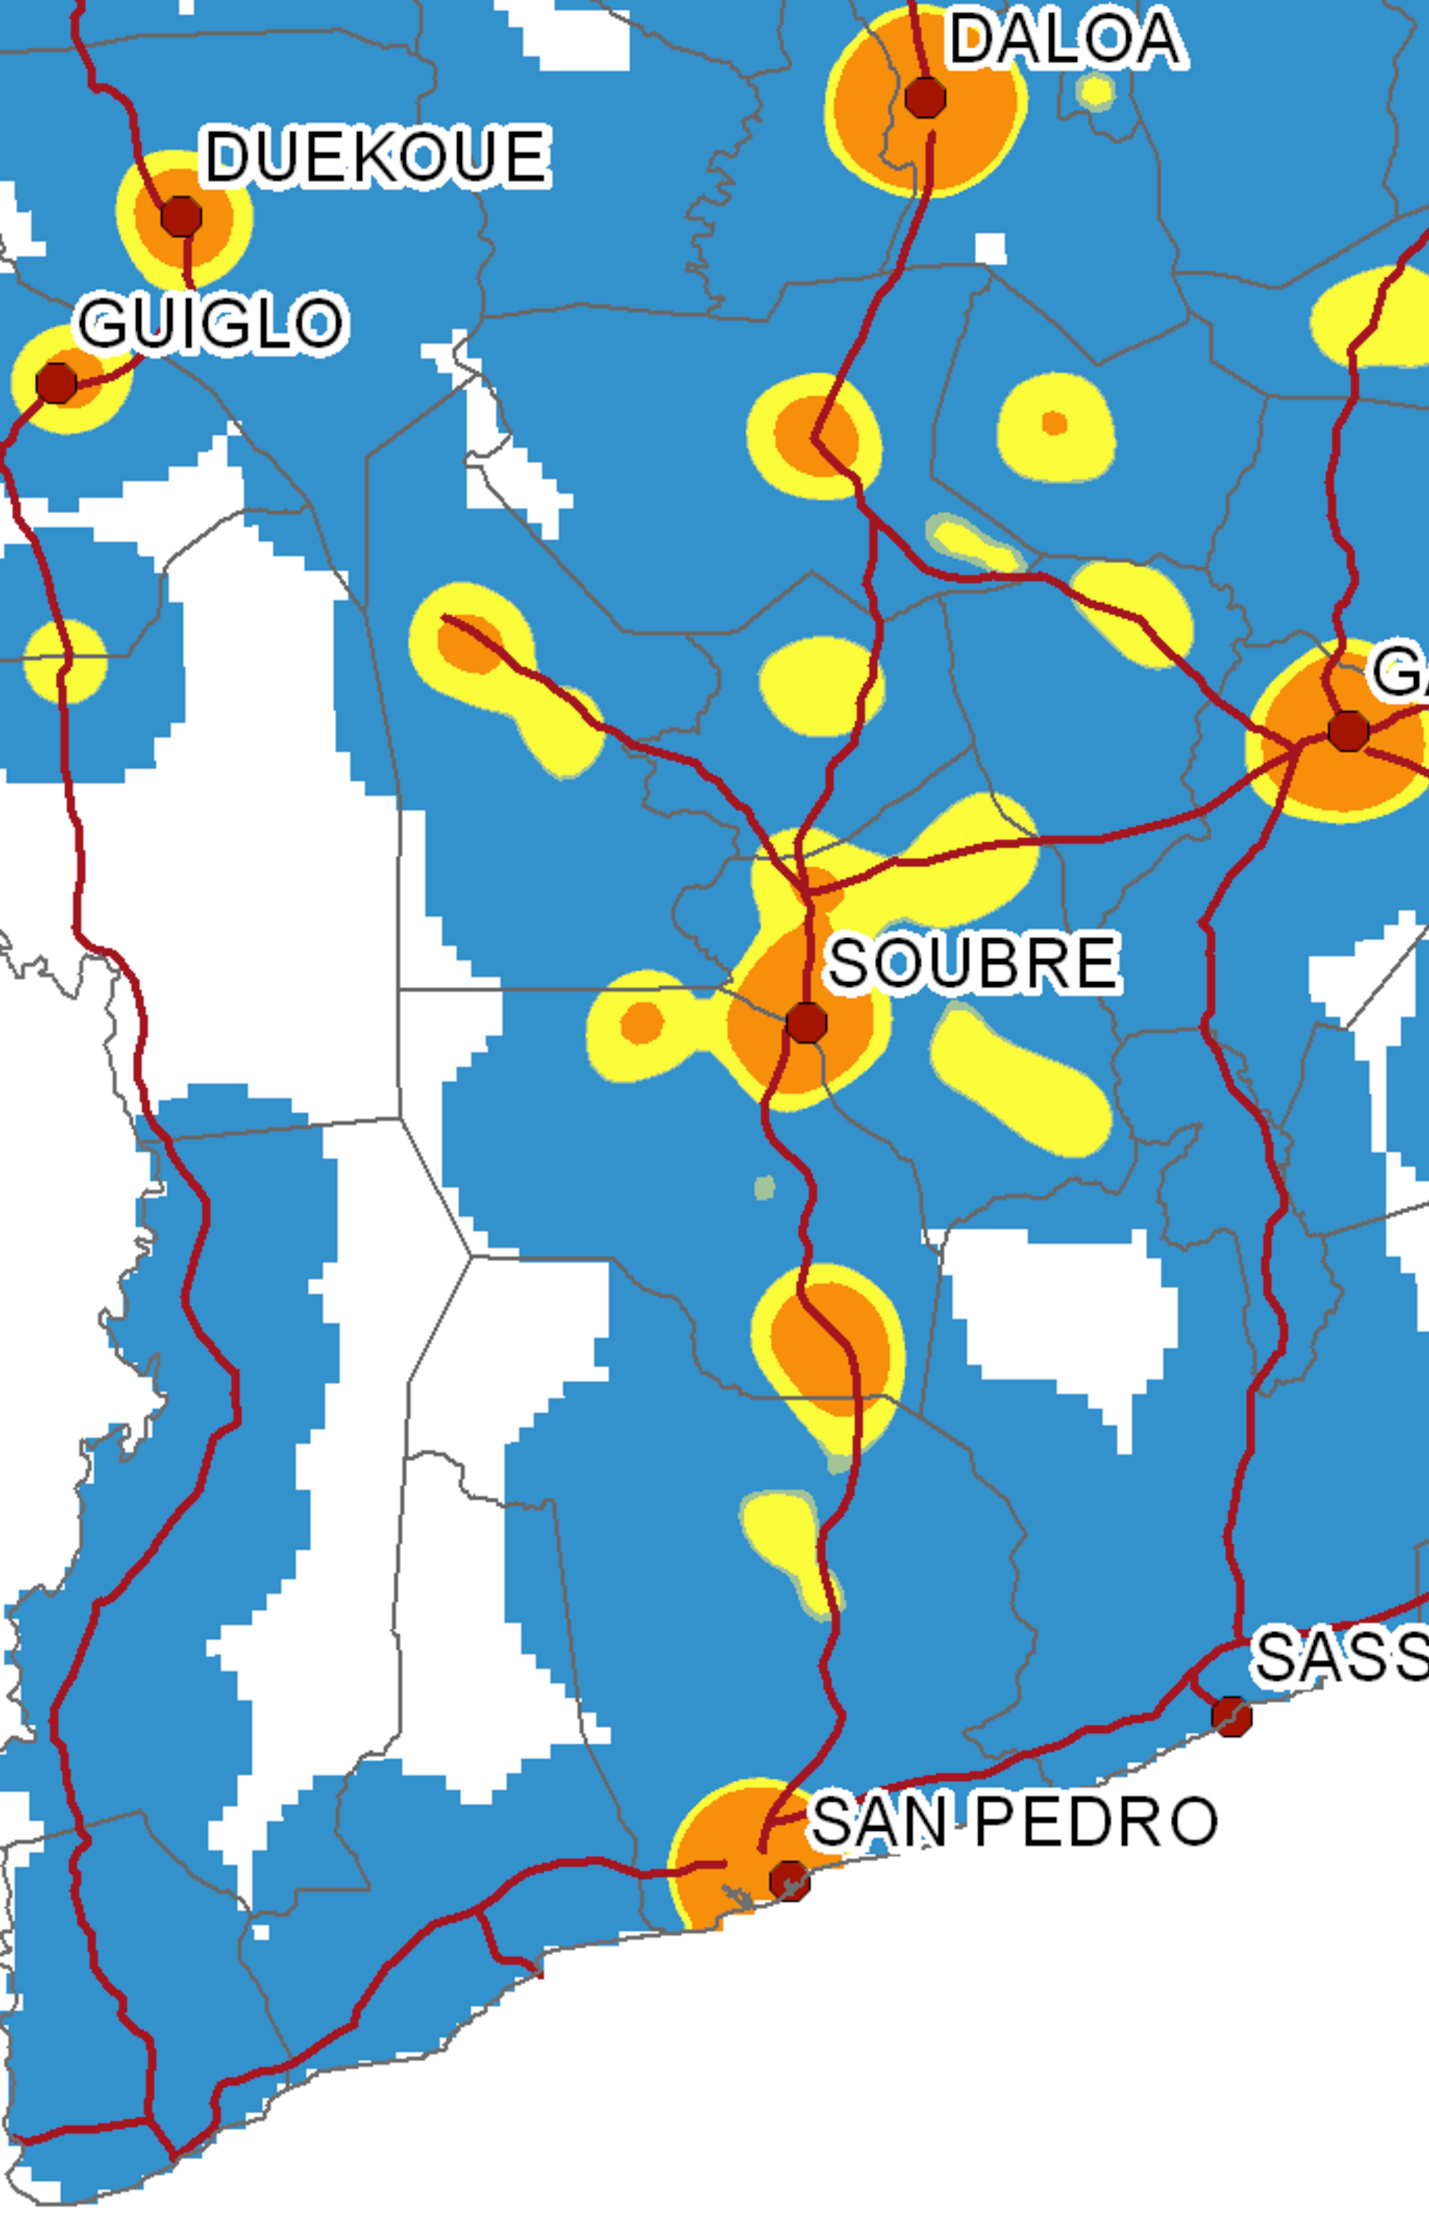
\includegraphics[scale = 0.1]{results/images/kernel/l_hour8_kd_detail.pdf}
	\label{fig:subfig2_detail}
}
\caption[KDE intensity dynamic when $p_1$ is reached and central valley starts]{KDE intensity smoothy when when  $p_1$ is reached}
\label{fig:subfigureExample}
\end{figure}


Therefore, the pictures above show the evolution of KDE in the focus location when maximum displacement $p_1$ is reached at 06:00, after this hour, KDE becomes softer at 07:00 and 08:00 starting the central valley. Through KDE  we can figure out that the median displacement in the central valley 08:00 and go on until $p_2$ has a greater value as numerical results leads.
\\
\\
The central valley has a uniform distribution of KDE and also we can observe in the next picture how the intensity increases when peak $p_2$ is reached. We propose the same location to explore and correlate the numerical results of $p_2$ with the final visualization of the dynamic taking into account the two variables.



\begin{figure}[h!]
\centering
\subfigure[Wednesday, 17:00]{
    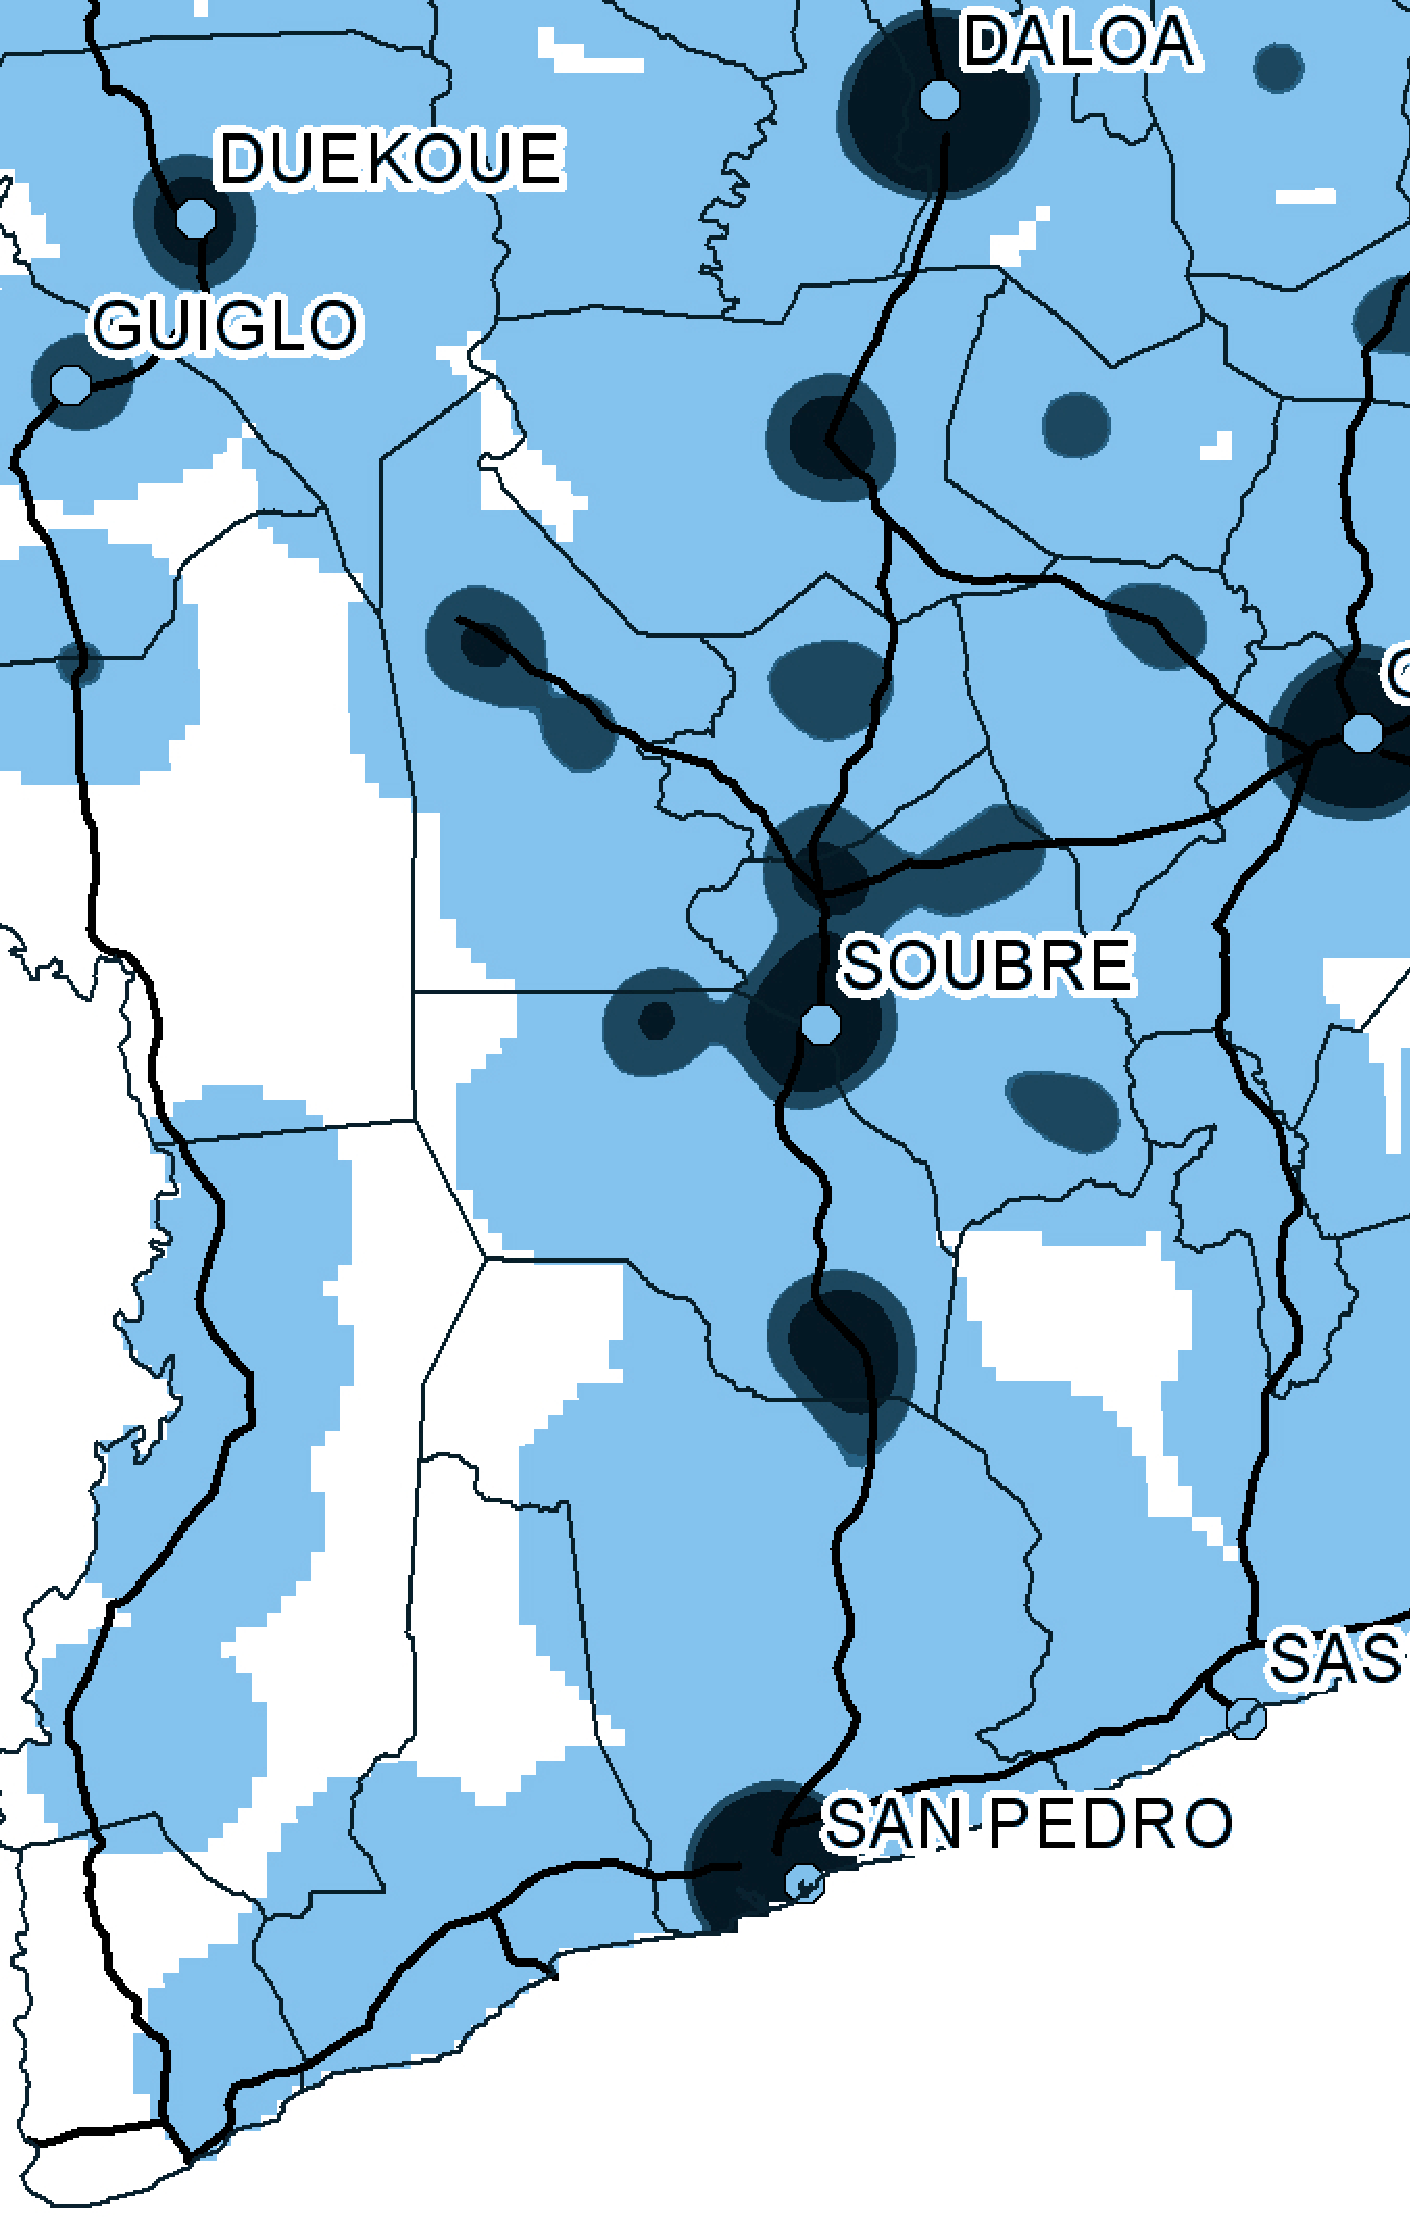
\includegraphics[scale = 0.1]{results/images/kernel/l_hour17_kd_detail.pdf}
	\label{fig:subfig1_detail}
}
\subfigure[Wednesday, 18:00]{
    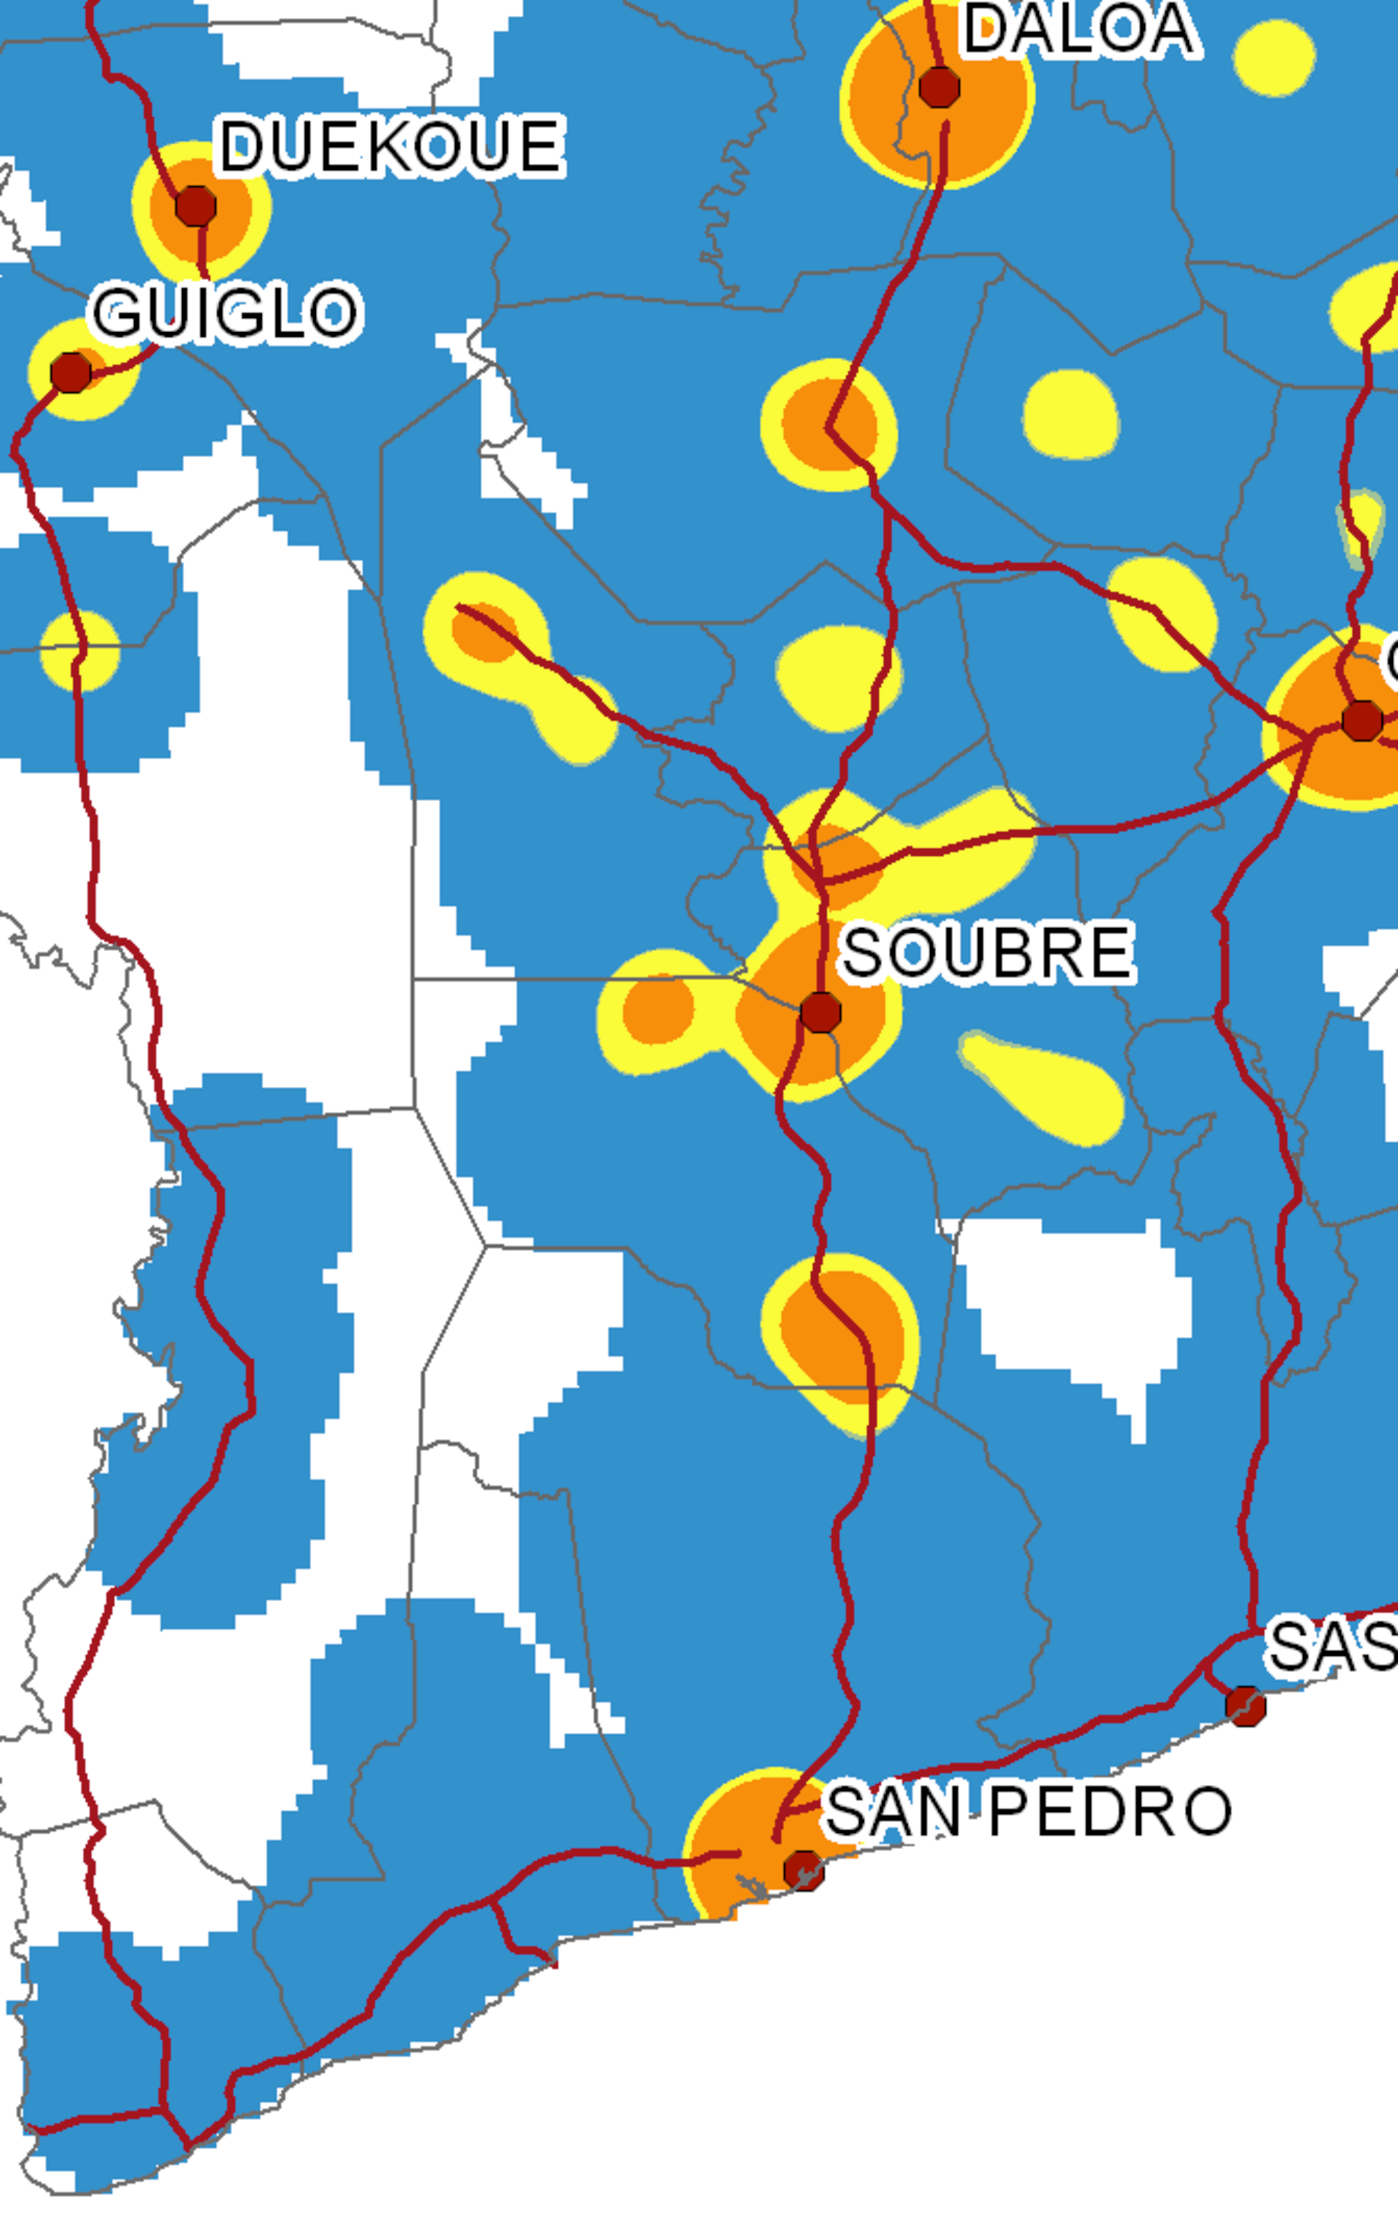
\includegraphics[scale = 0.1]{results/images/kernel/l_hour18_kd_detail.pdf}
	\label{fig:subfig2_detail}
}
\subfigure[Wednesday, 19:00]{
    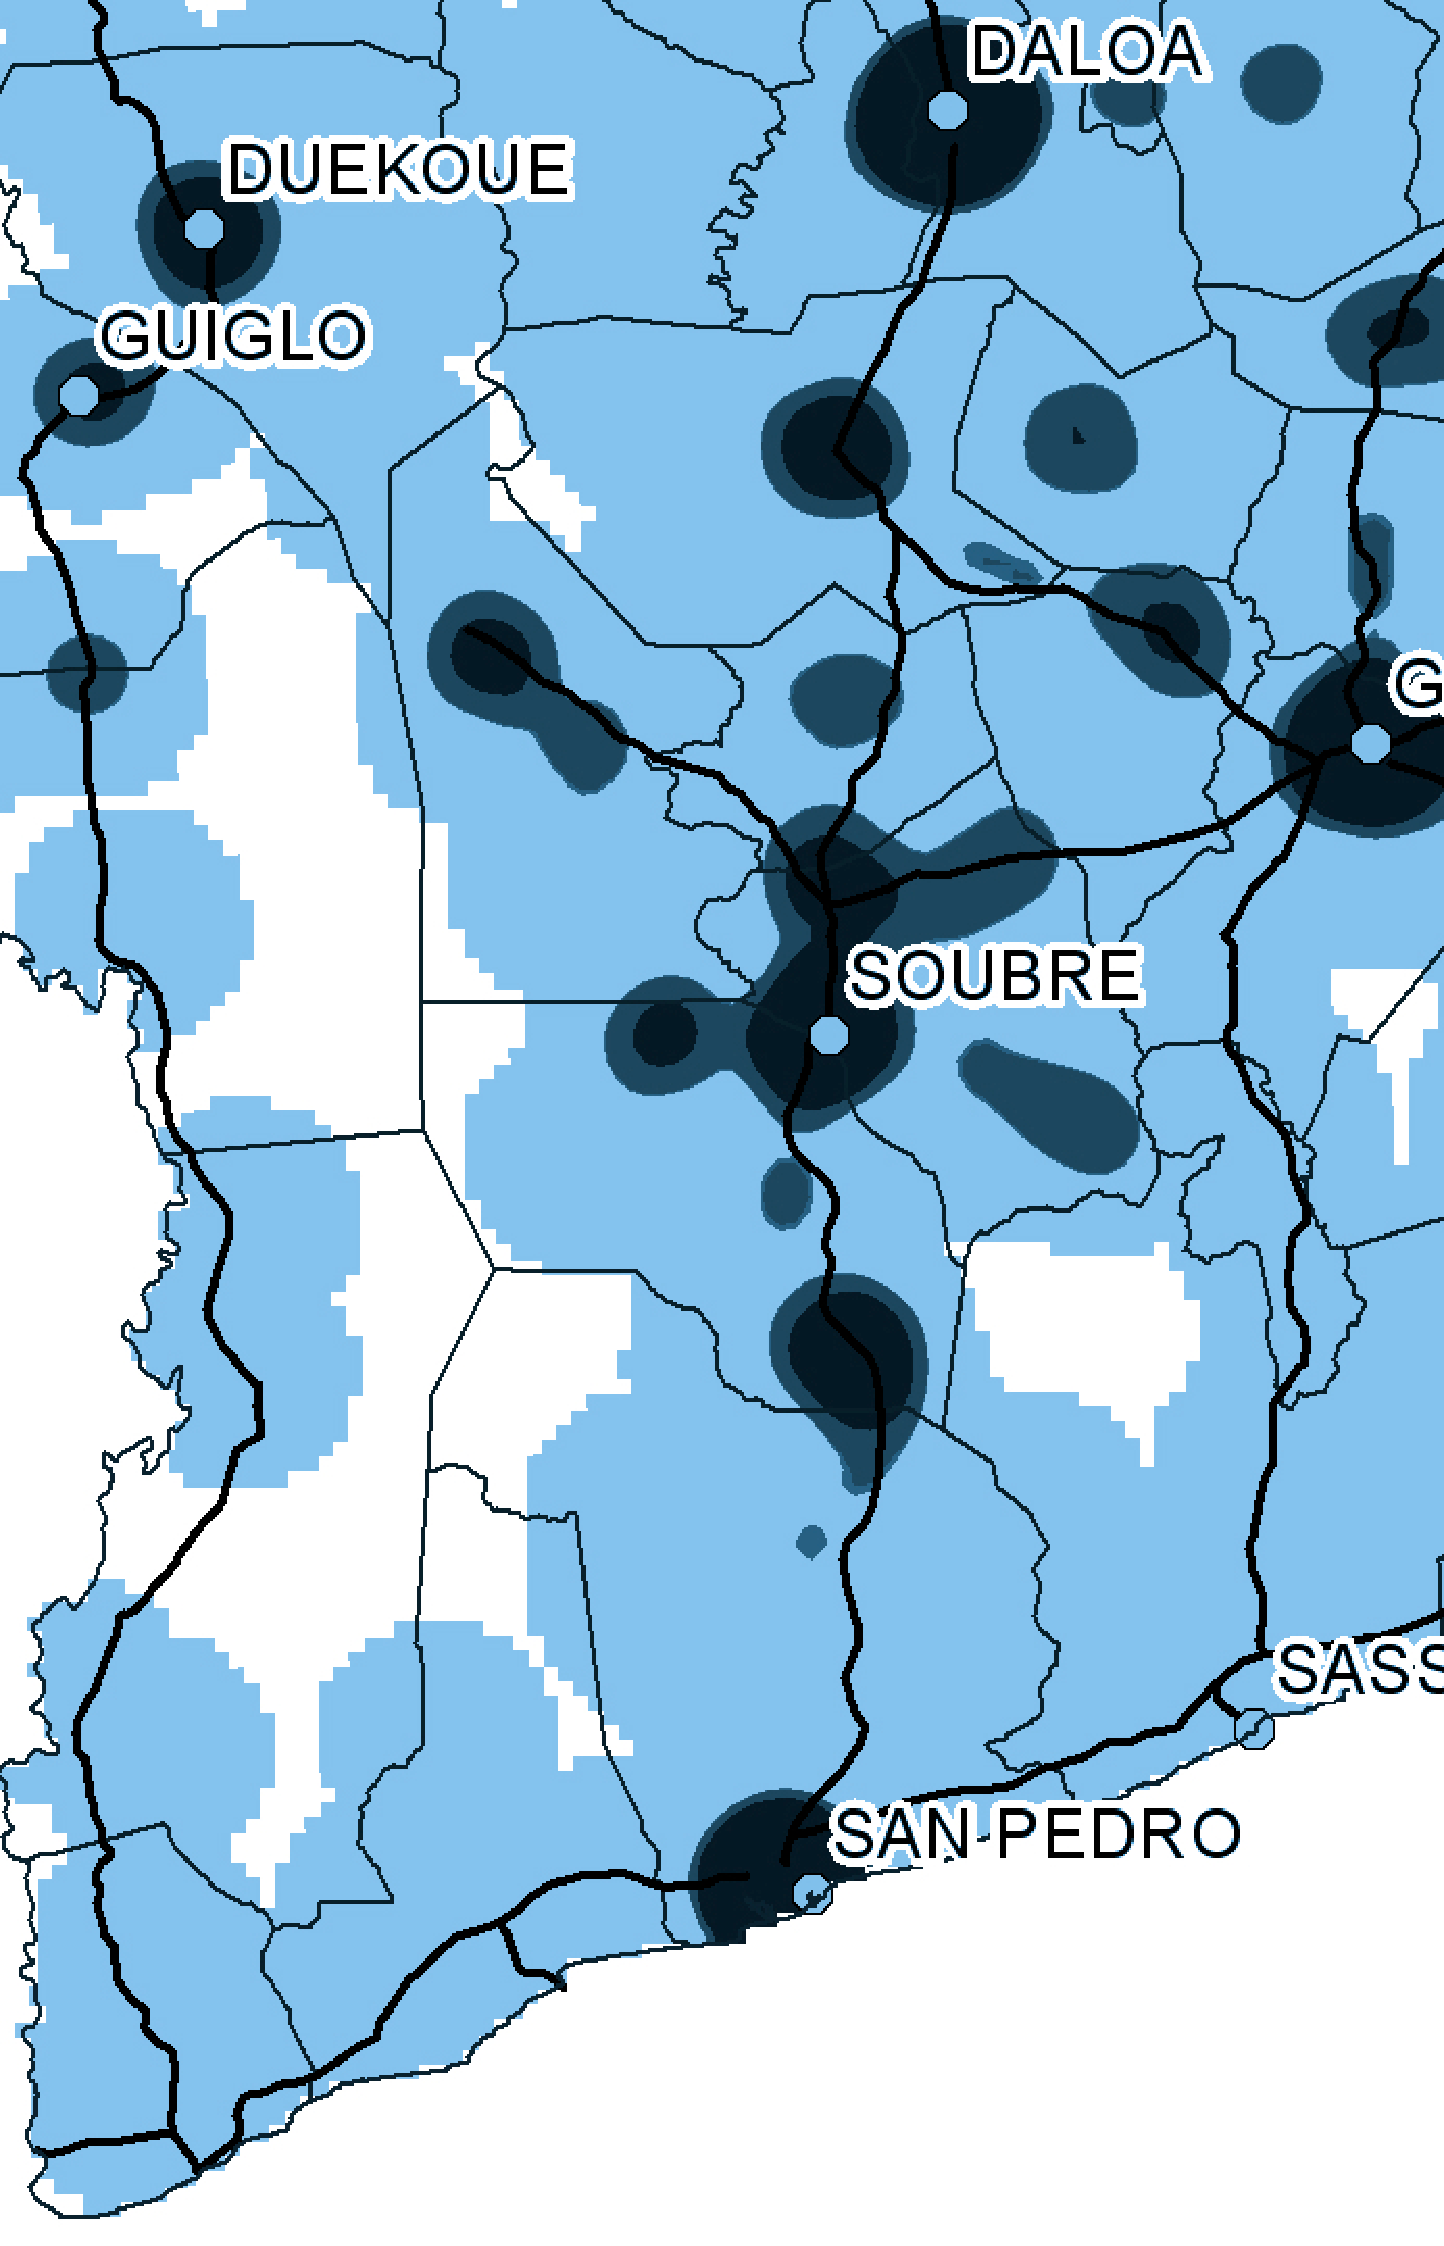
\includegraphics[scale = 0.1]{results/images/kernel/l_hour19_kd_detail.pdf}
	\label{fig:subfig2_detail}
}
\subfigure[Wednesday, 10:00]{
    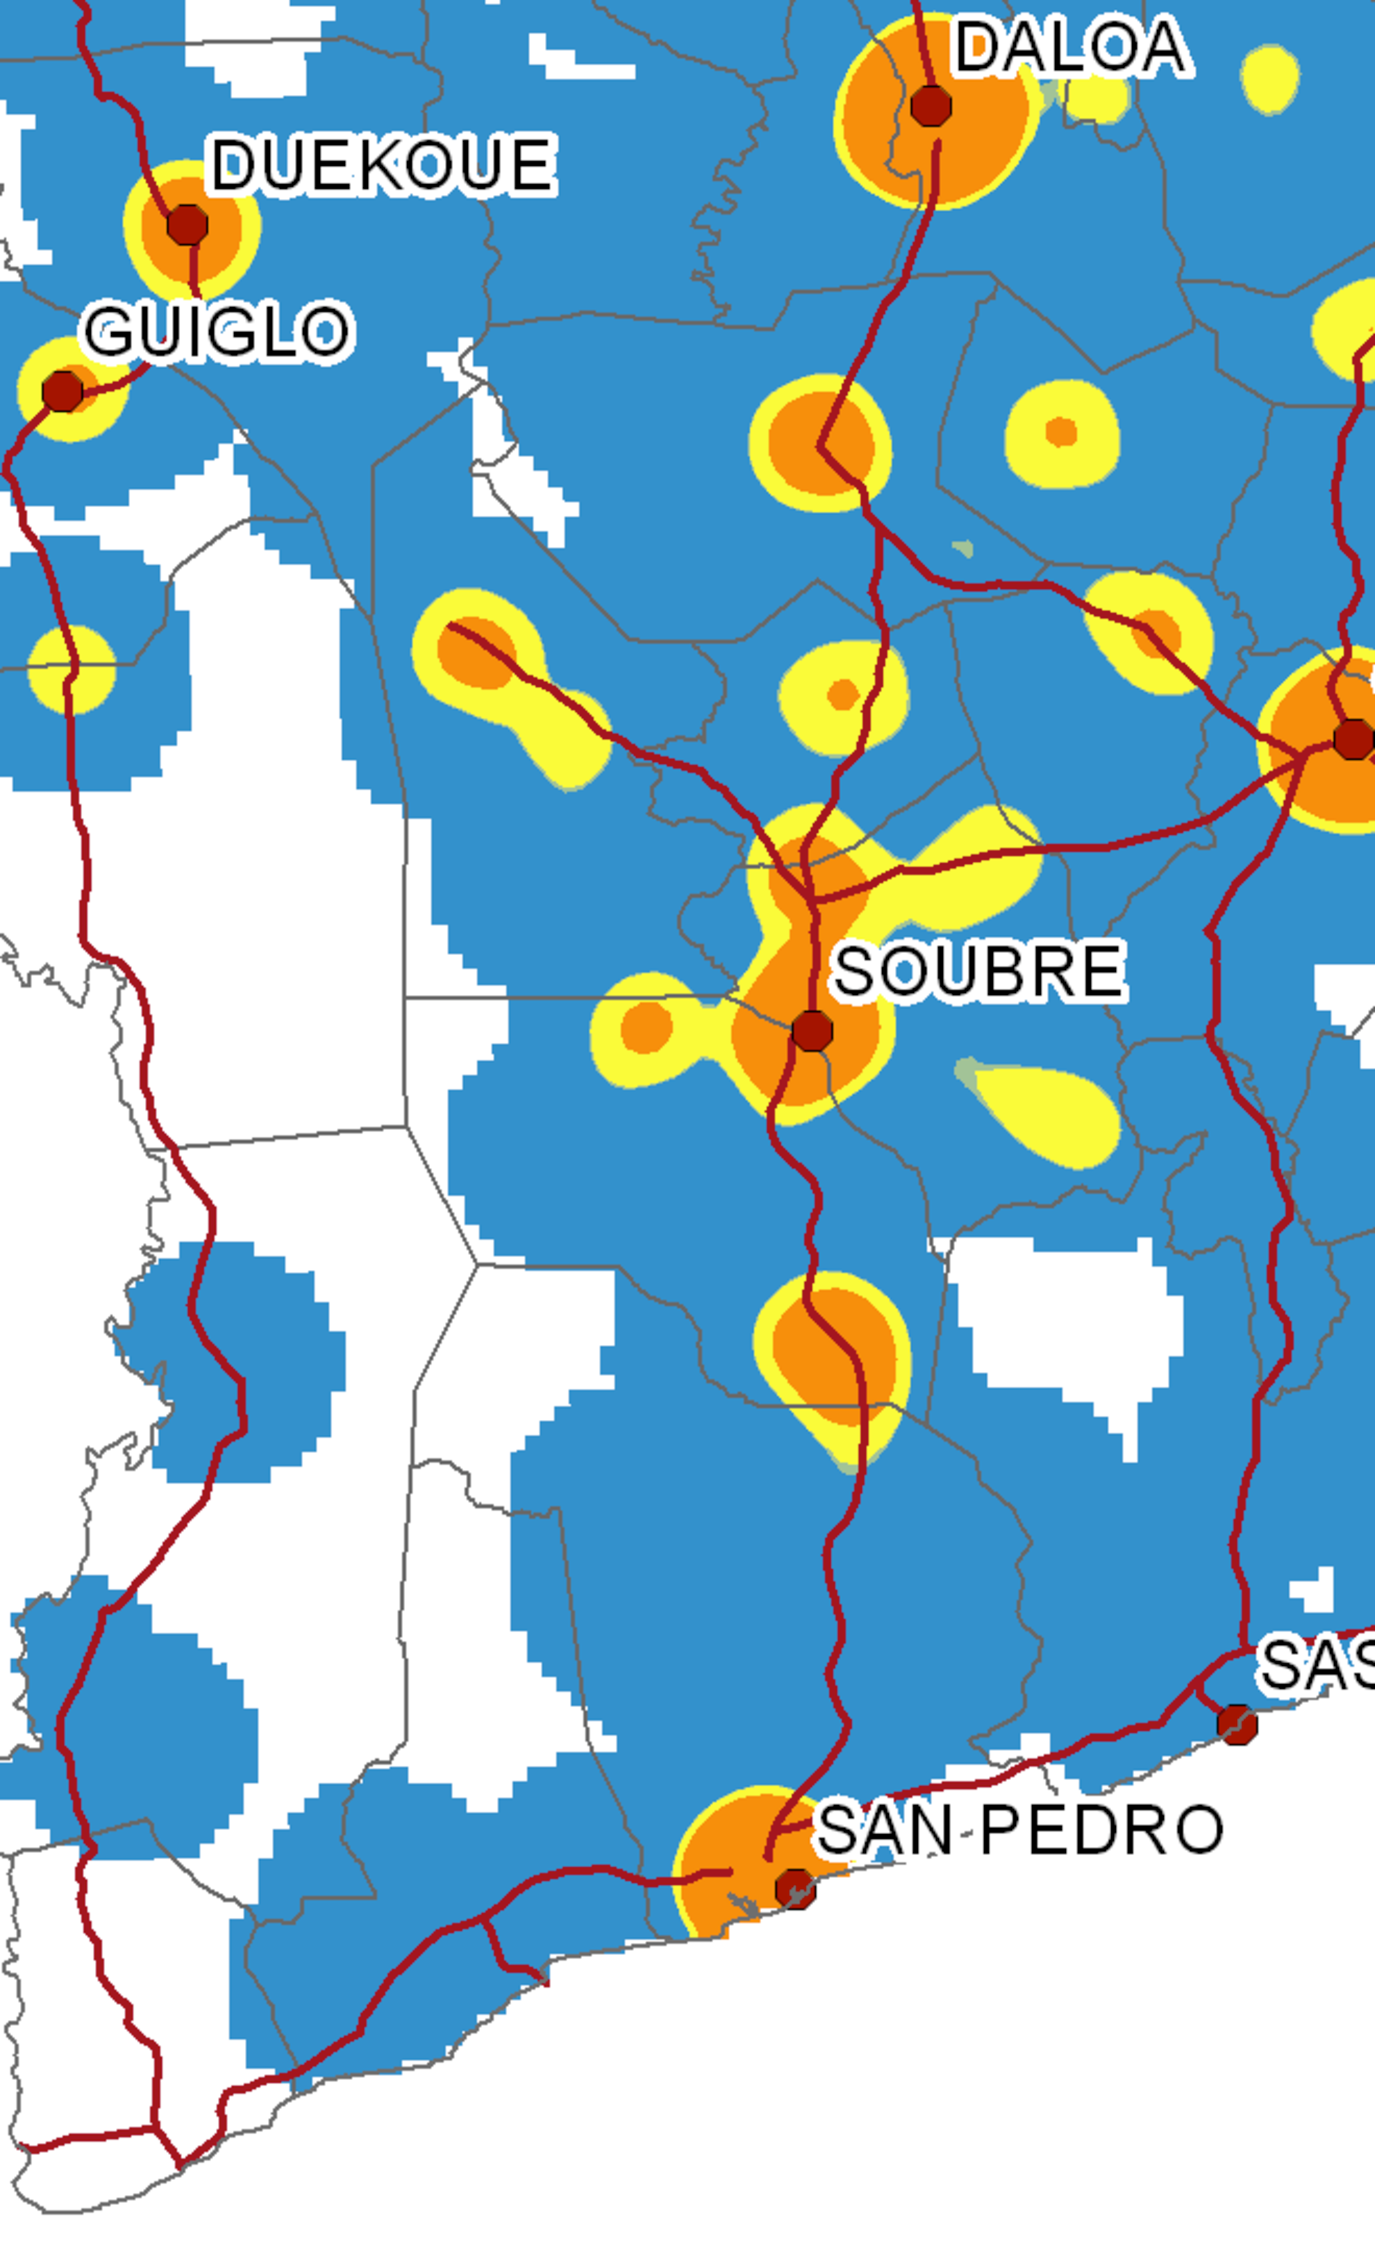
\includegraphics[scale = 0.1]{results/images/kernel/l_hour20_kd_detail.pdf}
	\label{fig:subfig2_detail}
}
\caption[KDE intensity smoothy when $p_2$ is reached]{KDE intensity smoothy when when  $p_2$ is reached}
\label{fig:subfigureExample}
\end{figure}




\newpage

\begin{figure}
\centering
\subfigure[Monday, 16:00]{
    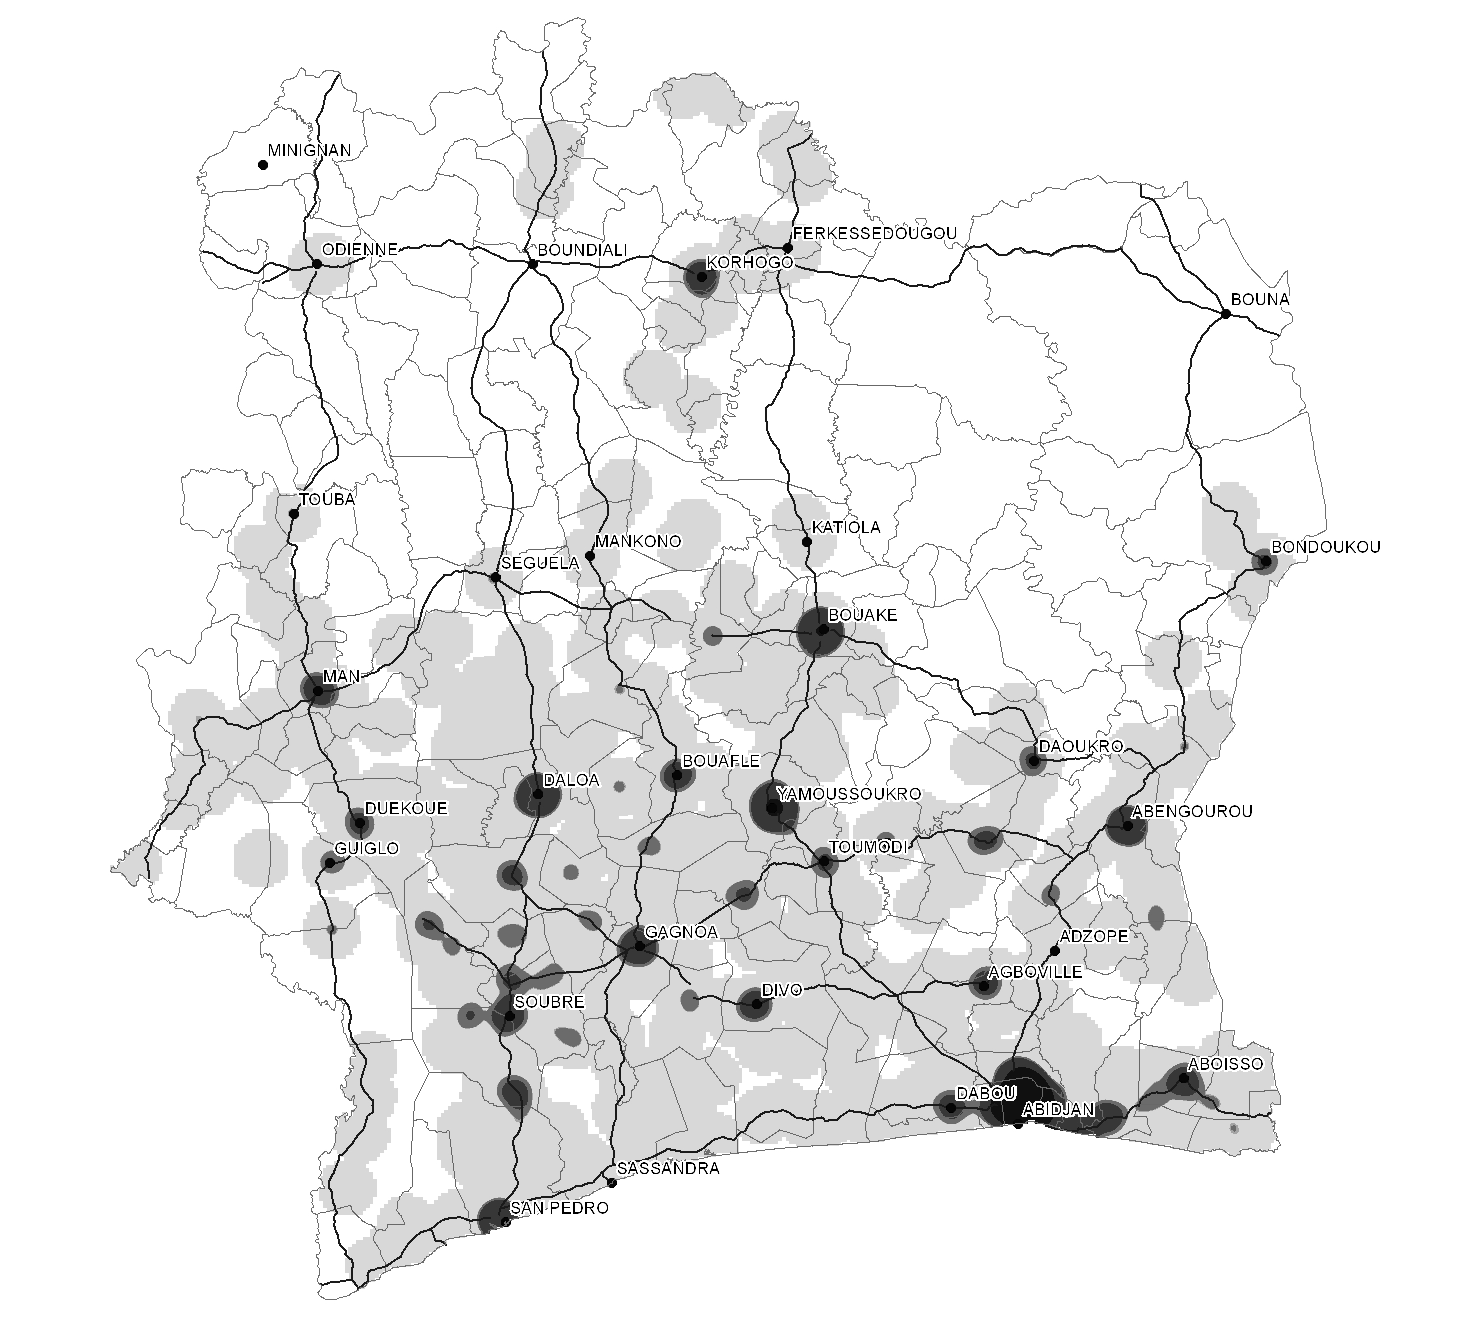
\includegraphics[scale = 0.3]{results/images/kernel/l_hour17_kd.pdf}
	\label{fig:subfig1}
}
\subfigure[Monday, 17:00]{
    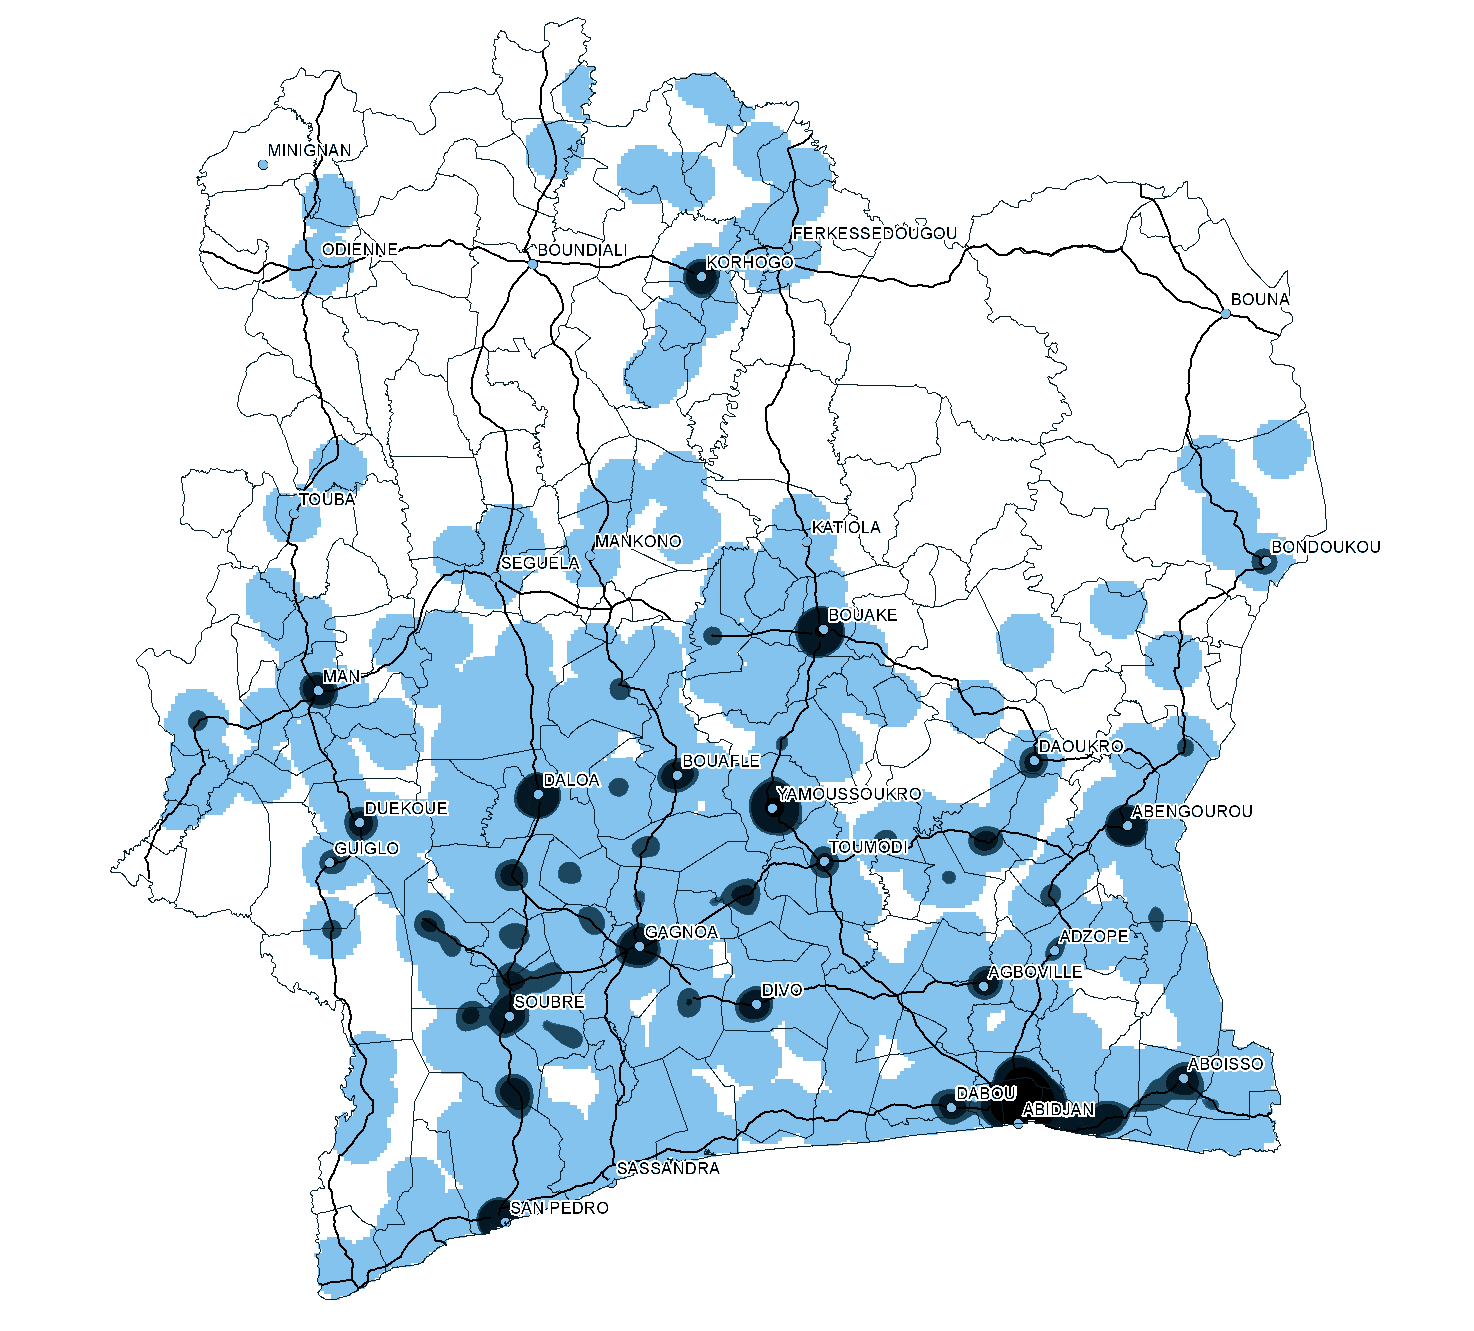
\includegraphics[scale = 0.3]{results/images/kernel/l_hour18_kd.pdf}
	\label{fig:subfig2}
}
\\
\subfigure[Monday, 18:00]{
    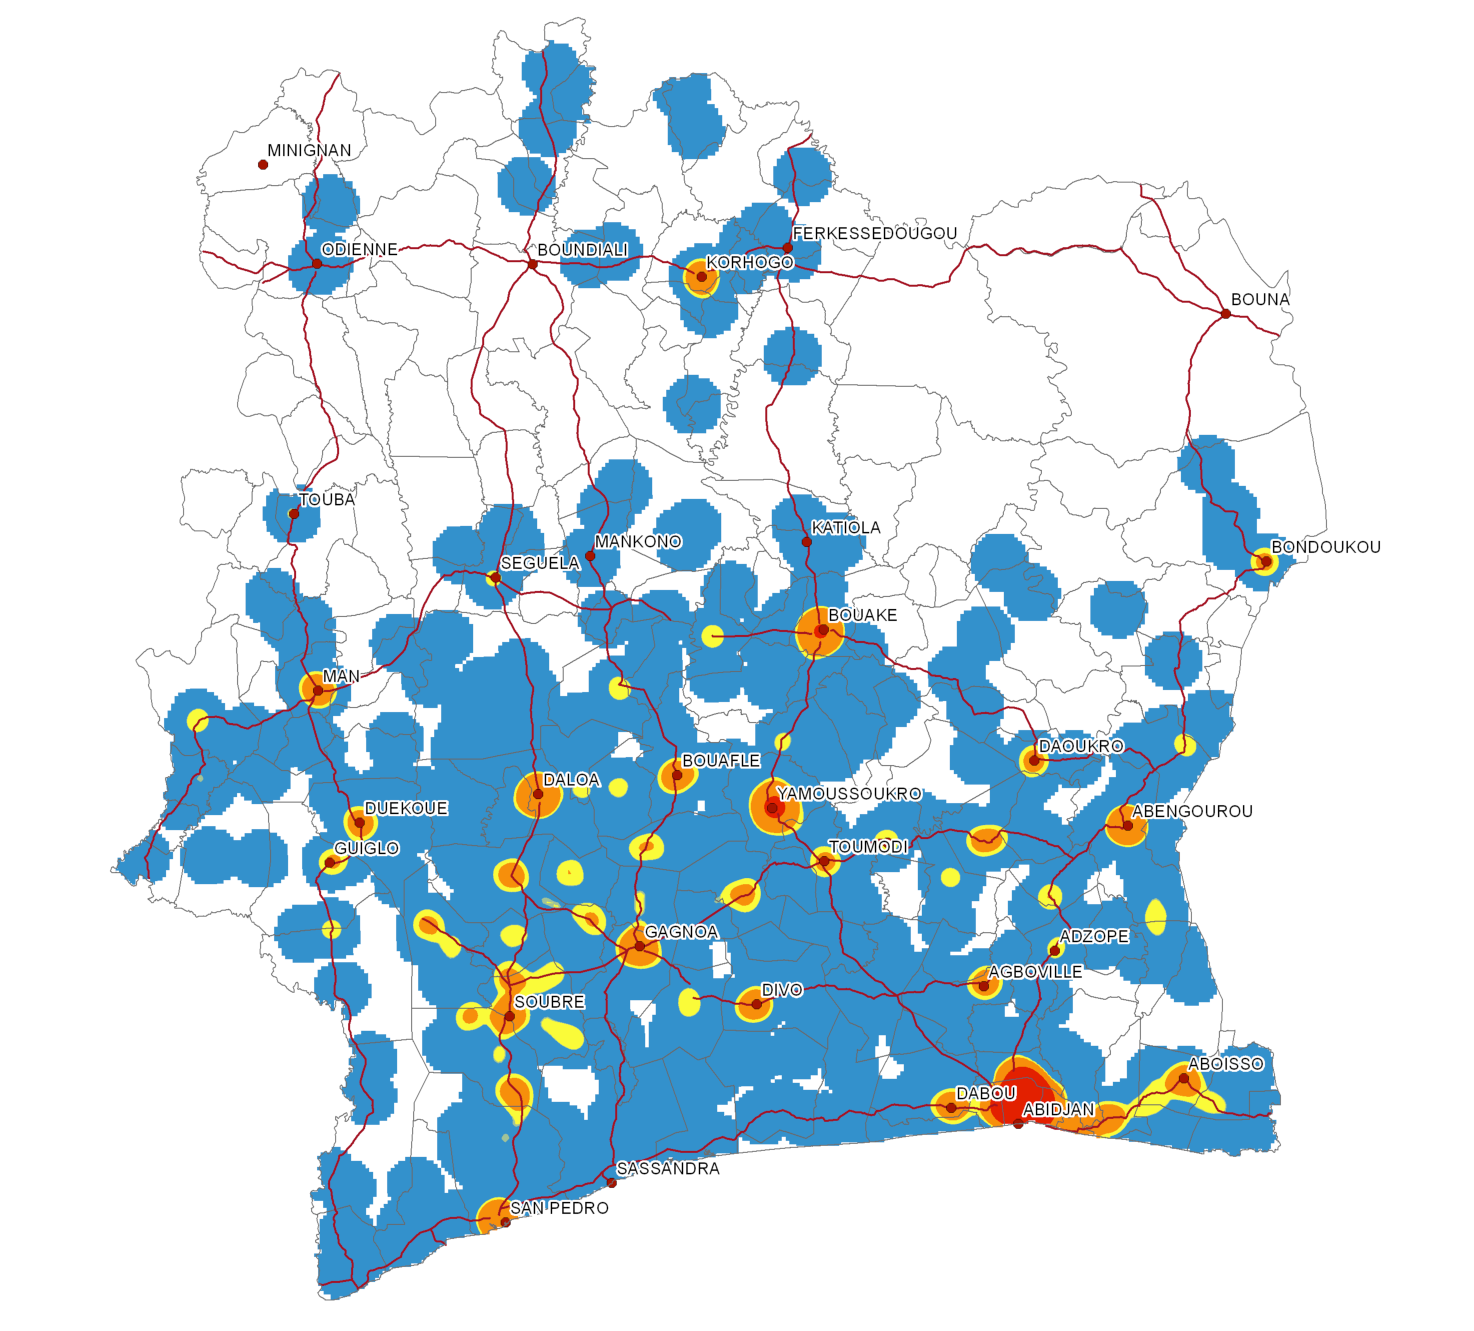
\includegraphics[scale = 0.3]{results/images/kernel/l_hour19_kd.pdf}
	\label{fig:subfig1}
}
\subfigure[Monday, 19:00]{
    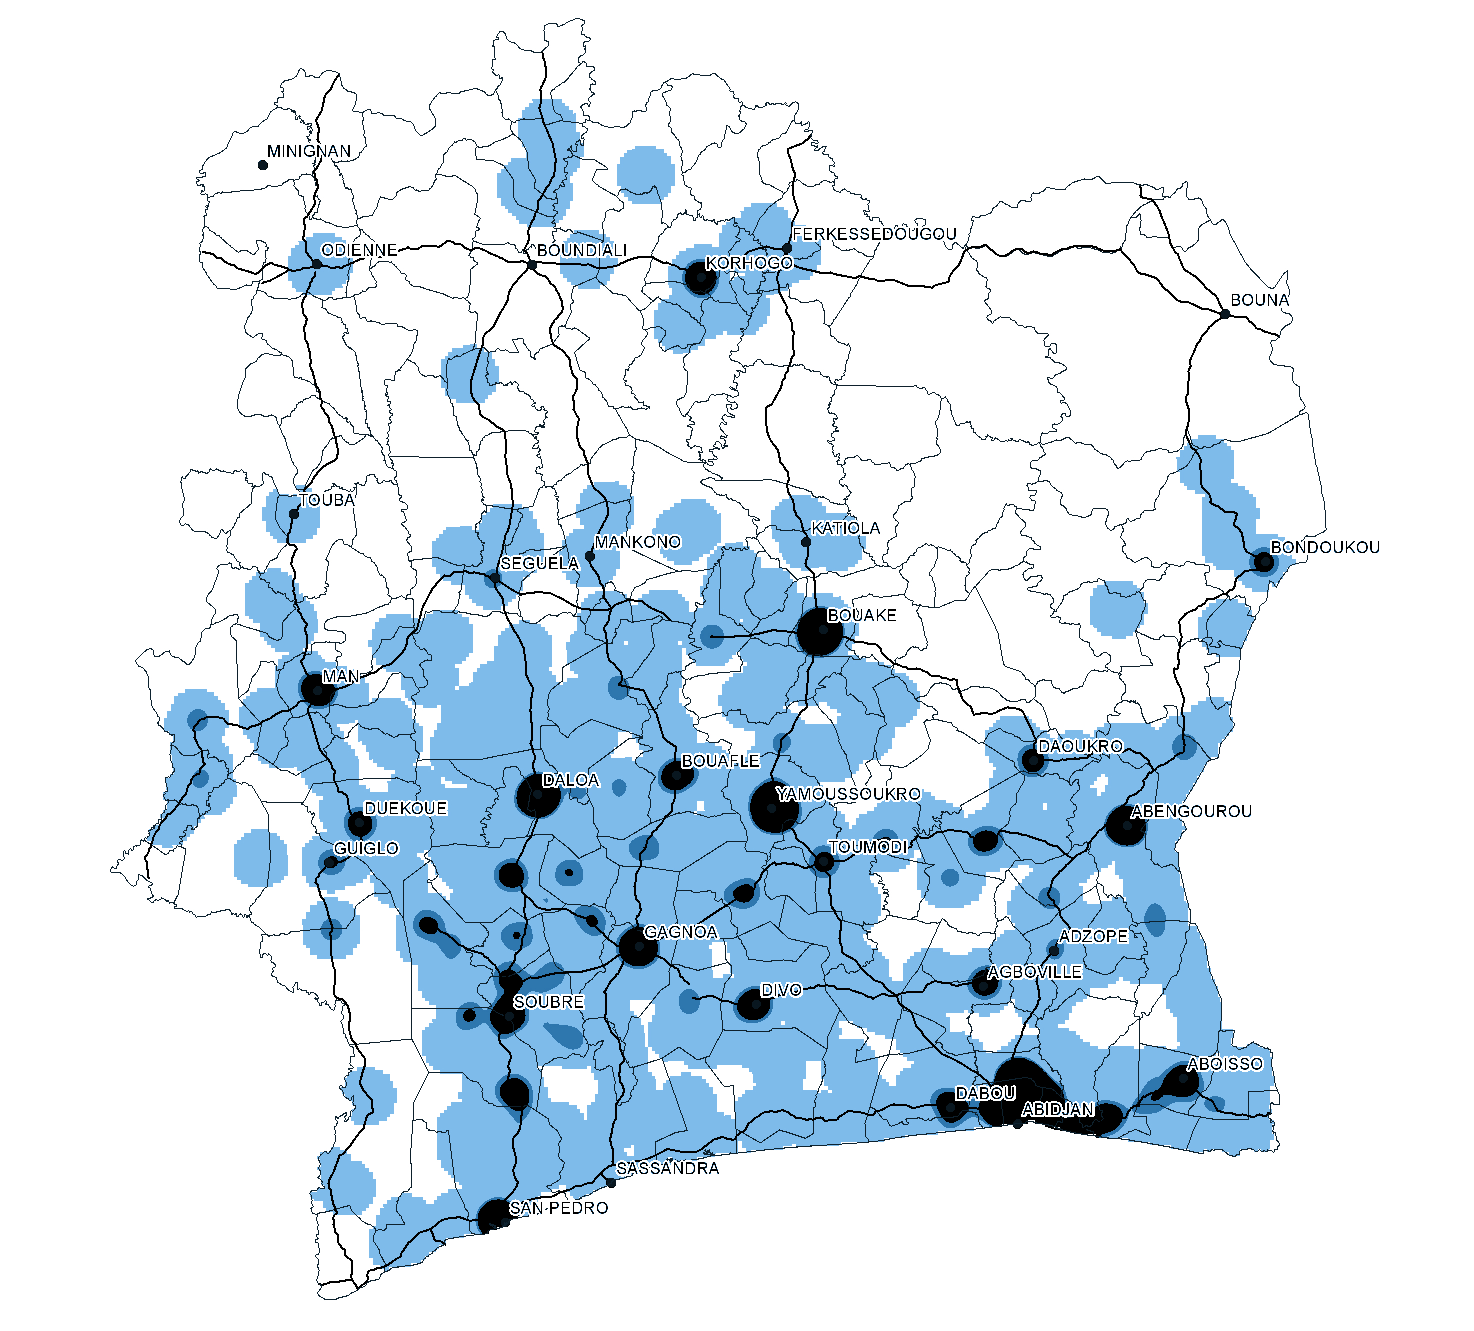
\includegraphics[scale = 0.3]{results/images/kernel/l_hour20_kd.pdf}
	\label{fig:subfig2}
}
\caption[KDE evolution while peak $p_1$ is reached]{Evolution of KDE while peak $p_2$ is reached}
\label{fig:subfigureExample}
\end{figure}






